\documentclass[12pt,a4paper]{article}
\usepackage[latin1]{inputenc}
\usepackage[english]{babel}
\usepackage{amsmath}
\usepackage{amsfonts}
\usepackage{amssymb}
\usepackage{makeidx}
\usepackage{lmodern}
\usepackage{fourier}
\usepackage{listings}
\usepackage{calc,xcolor} 
\usepackage{subfigure}

\usepackage{calc}
%
\usepackage{flowchart} % also loads tikz
\usepackage{tikz}
\usetikzlibrary{arrows}
%\usepackage{pgflibraryarrows}



%
\definecolor{hellgelb}{rgb}{1,1,0.8}
\definecolor{colKeys}{rgb}{0,0,1}
\definecolor{colIdentifier}{rgb}{0,0,0}
\definecolor{colComments}{rgb}{1,0,0}
\definecolor{colString}{rgb}{0,0.5,0}

\lstset{%
    float=hbp,%
    basicstyle=\ttfamily\small, %
    identifierstyle=\color{colIdentifier}, %
    keywordstyle=\color{colKeys}, %
    stringstyle=\color{colString}, %
    commentstyle=\color{colComments}, %
    columns=flexible, %
    tabsize=2, %
    frame=single, %
    extendedchars=true, %
    showspaces=false, %
    showstringspaces=false, %
    numbers=left, %
    numberstyle=\tiny, %
    breaklines=true, %
    backgroundcolor=\color{hellgelb}, %
    breakautoindent=true, %
    captionpos=b%
}

\usepackage{float} 
\newfloat{Listing}{hbp}{lis}[section]

\definecolor{MyGray}{rgb}{0.96,0.97,0.98}
\makeatletter\newenvironment{graybox}{%
   \noindent\begin{lrbox}{\@tempboxa}\begin{minipage}{\textwidth}}{\end{minipage}\end{lrbox}%
   \colorbox{MyGray}{\usebox{\@tempboxa}}
}\makeatother

\newcommand{\MueLu}{MueLu}
\newcommand{\Xpetra}{Xpetra}

\author{Tobias Wiesner}
\begin{document}

\section{Tutorial 1}
Welcome to \MueLu, the next generation multigrid package in Trilinos.

\MueLu~ is meant to be the successor package of the ML Trilinos package, which implements a smoothed aggregation based algebraic Multigrid method. \MueLu~ is designed as a framework that is flexible enough not only to provide smoothed aggregation based algebraic multigrid but also Ruge-Stueben AMG or even geometric multigrid methods\footnote{Note, that MueLu is still in an early phase of development and only has a smoothed aggregation AMG method implemented yet.}.

%Based on a very modern software framework it provides easy-to-use XML interfaces for the user.

\paragraph{Preparation for hands-on tutorial}
To compile the test programs, you first have to run the configuration script, that prepares the compilation on your computer. Just open a terminal, change to the folder with the text examples and type \verb|./do-configure|. Usually you have to do this step only once in the beginning.

After the configuration process you can compile the test programs by typing \verb|make|. The compiler now should generate the executables \verb|MueLu_laplace2d.exe|, \verb|MueLu_recirc2d.exe| and \verb|MueLu_recirc2d_api.exe|. 

For visualization purposes make sure, that python is installed on your machine with the VTK bindings. Furthermore \verb|paraview| is needed for displaying the multigrid aggregates (optional) and \verb|gnuplot| is needed for plotting the solutions.

\section{Tutorial 2}

\subsection{Test example}
We generate a test matrix corresponding to the stencil of a 2D Laplacian operator on a structured Cartesian grid. The matrix stencil is
\begin{displaymath}
\frac{1}{h^2}\begin{pmatrix} & -1 & \\ -1 & 4 & -1 \\ & -1 & \end{pmatrix}.
\end{displaymath}
The resulting matrix is symmetric positive definite. We choose the right hand side to be the constant vector one and use a random initial guess for the iterative solution process. The problem domain is the unit cube with a Cartesian (uniform) mesh.

%\subsection{Test program}

\subsection{XML Interface}

\begin{Listing} 
\begin{center} 
\begin{lstlisting}[language=XML,label=listing:SAAMGXML]
<ParameterList name="MueLu">
  <ParameterList name="Matrix">
    <Parameter name="PDE equations" type="int" value="1"/> 
  </ParameterList>

  <!-- Factory collection -->
  <ParameterList name="Factories">
     
    <ParameterList name="myJacobi">
      <Parameter name="factory" type="string" value="TrilinosSmoother"/>
      <Parameter name="type" type="string" value="RELAXATION"/>
      <ParameterList name="ParameterList">
       <Parameter name="relaxation: type" type="string" value="Jacobi"/>
       <Parameter name="relaxation: sweeps" type="int"    value="1"/>
       <Parameter name="relaxation: damping factor" type="double" value="0.9"/>
      </ParameterList>
    </ParameterList>
   </ParameterList>

  <!-- Definition of the multigrid preconditioner -->
  <ParameterList name="Hierarchy">

    <Parameter name="numDesiredLevel" type="int" value="1"/> 
    <Parameter name="maxCoarseSize" type="int" value="10"/>
    <Parameter name="verbosity" type="string"   value="Low"/>

    <ParameterList name="All">
     <Parameter name="Smoother" type="string" value="myJacobi"/>
     <Parameter name="CoarseSolver" type="string"   value="myJacobi"/>    
    </ParameterList>
  </ParameterList>
</ParameterList>
\end{lstlisting}
\caption{Structure of XML input file for \MueLu~ with smoothed aggregation transfer operators and Jacobi level smoothers.} 
\label{listing:SAAMGXML}
\end{center}
\end{Listing}

\paragraph{Step 1: Start with one-level method.}
Before we apply a multigrid method as solver, let's start with simple Jacobi sweeps and have a look at the error.
By setting the maximum multigrid levels to 1 and using a Jacobi smoother as coarse solver we obtain a pseudo multigrid method which corresponds to a simple Jacobi iteration. Listing \ref{listing:SAAMGXML} gives the multigrid XML parameters for the 1 level dummy multigrid method. Figures \ref{fig:2dlap111} to \ref{fig:2dlap11100} as well as figures \ref{fig:2dlap511} to \ref{fig:2dlap51100} show the smoothing effect of the Jacobi iteration.

\begin{graybox}
 \textbf{Exercise}
 \begin{itemize}
 \item Run the test program using the solver parameters from listing% \ref{listing:SAAMGXML}.
       \begin{verbatim}
       ./MueLu_laplace2d.exe --xml=xml/s2a.xml
       \end{verbatim}
       Note, that \verb|./MueLu_laplace2d.exe --help| prints all available options. Use \verb|mpirun| to run the program in parallel, e.g. on 2 processors
       \begin{verbatim}
       mpirun -np 2 ./MueLu_laplace2d.exe --xml=xml/s2a.xml
       \end{verbatim}
 \item For visualization of the output use the \verb|hands-on.sh| script. Run the script with
       \begin{verbatim}
       ./hands-on.sh
       \end{verbatim}
       and choose option 1 for the 2D Laplace example on a $50\times 50$ mesh. Then, the output is
       \begin{verbatim}
=== 2D Laplace (50 x 50) === 

 solver: procs: 2 Multigrid sweeps: 1


1) rerun example              7) plot exact solution
2) change multigrid sweeps    8) plot Multigrid solution
3) change mesh                9) plot error
4) change solver             10) plot proc distribution
5) change procs              11) Quit
6) show output
       \end{verbatim}
       Select option 6 to print the output of the \verb|MueLu_laplace2d.exe| program on screen. With \verb|q| you return to above menu. Option 7 plots the exact solution, that has been calculated with a direct solver. Option 8 plots the approximate solution after one sweep with the multigrid V cycle. Option 9 plots the error (the difference of the exact solution and the approximate multigrid solution).
 \end{itemize}
 \end{graybox}

\paragraph{Step 2: Increase number of multigrid levels.}
The next step is to increase the number of multigrid levels. We begin with a 2 level multigrid method. We choose the parameters \texttt{numDesiredLevel} and \texttt{maxCoarseSize} accordingly such that a 2 level multigrid hierarchy is built. The parameter \texttt{maxCoarseSize} defines the size of the coarse level problem (number of matrix rows of the coarsest system) before the multigrid coarsening is stopped. Again we use Jacobi iterations as level smoothers on all multigrid levels with a fixed damping parameter $\omega=0.9$.
As one can see from figures  \ref{fig:2dlap121} to \ref{fig:2dlap12100} the error is reduced more efficiently when using more multigrid levels. A too high number of level smoothing sweeps with Jacobi gives no significant improvement.

\begin{graybox}
 \textbf{Exercise}
 \begin{itemize}
  \item Create a copy of the xml solver parameters in file \verb|xml/s2a.xml|, that you can adapt for your experiments.
        \begin{verbatim}
        cp xml/s2a.xml mysolver.xml
        \end{verbatim}
  \item Run the \verb|hands-on.sh| script, select option 1 for the 2D Laplace example. Then choose option 4 to change the used solver parameters and enter your chosen filename for your solver parameters file.
        \begin{verbatim}
=== 2D Laplace (50 x 50) === 

 solver: procs: 2 Multigrid sweeps: 1
 
1) rerun example              7) plot exact solution
2) change multigrid sweeps    8) plot Multigrid solution
3) change mesh                9) plot error
4) change solver             10) plot proc distribution
5) change procs              11) Quit
6) show output
Select: 4

*** 2D Laplace example ***

XML file=mysolver.xml
        \end{verbatim}
        The filename for the currently used solver parameters is also printed above the menu, such that you can check which solver parameter file is used.
   \item Edit your solver parameter file (e.g. \verb|mysolver.xml|) using your favorite text editor and adapt the parameters. Set the \texttt{numDesiredLevel} parameter to $2$ to obtain a two level multigrid method and choose a value for \texttt{maxCoarseSize} that is small enough that a 2 level multigrid hierarchy is built (e.g. 10). Don't forget to save your changes.
   \item Select the option 1 to rerun your example using the solver parameters from \verb|mysolver.xml| with your recent changes. Check the solver output and the plots. You can also increase the number of multigrid sweeps (using option 2) and see how the error changes.
%   \item Change your solver parameters for obtaining a three level multigrid method.
 \end{itemize}
\end{graybox}

\paragraph{Step 3: Use a direct solver on the coarsest grid.}
One of the core ideas of multigrid is to coarsen the fine level problem such that we can use a direct solver to obtain the exact coarse level solution with reasonable costs. In the \texttt{CoarsestLevel} section we change the value of the parameter \texttt{CoarseSolver} to \textit{DirectSolver}. That is, we use Jacobi sweeps as pre- and postsmoother on the finest and the intermedium levels and a direct solve on the coarsest level.
In figures \ref{fig:jacobisolver} and \ref{fig:directsolver} one can compare the output of the multigrid setup either when using Jacobi sweeps as coarse level smoothers or a direct solver. One can also see, that a direct solver has some beneficial effects when the multigrid method is used as preconditioner within CG. The number of linear iterations is reduced from 10 iterations to 7 iterations.

\begin{graybox}
 \textbf{Exercise}
 \begin{itemize}
  \item Run the \verb|hands-on.sh| script, select option 1 for the 2D Laplace example. Then choose option 4 to change the used solver parameters and enter your chosen filename for your solver parameters file.
  \item Change your solver parameters for obtaining a three level multigrid method. Furthermore change the parameter \verb|CoarseSolver| in the \verb|CoarsestLevel| section from \verb|myJacobi| to \verb|DirectSolver|. Then, on the coarsest level a direct solver is used (KLU) instead of the Jacobi sweep defined in the \verb|myJacobi| section. Don't forget to save your changes and to rerun the example.    
  \item Check the difference in the output of the multigrid setup.
 \end{itemize}
\end{graybox}

\begin{figure}
\tiny
\begin{minipage}{\textwidth}
\begin{verbatim}
 --------------------------------------------------------------------------------
 ---                            Multigrid Summary                             ---
 --------------------------------------------------------------------------------
 Number of levels    = 3
 Operator complexity = 1.36
 Max Coarse Size     = 10
 Implicit Transpose  = false
 
 matrix rows    nnz  nnz/row procs
 A 0    2500  12300     4.92  2
 A 1     442   3870     8.76  2
 A 2      60    520     8.67  2
 
 Smoother (level 0) both : MueLu::IfpackSmoother{type = point relaxation stand-alone}
 
 Smoother (level 1) both : MueLu::IfpackSmoother{type = point relaxation stand-alone}
 
 Smoother (level 2) pre  : MueLu::IfpackSmoother{type = point relaxation stand-alone}
 Smoother (level 2) post :  no smoother
 
Use multigrid hierarchy as preconditioner within CG.

                *******************************************************
                ***** Problem: Epetra::CrsMatrix
                ***** Preconditioned CG solution
                ***** MueLu::Hierarchy
                ***** No scaling
                *******************************************************

                iter:    0           residual = 1.000000e+00
                iter:    1           residual = 1.412917e-02
                iter:    2           residual = 1.015400e-03
                iter:    3           residual = 5.716660e-04
                iter:    4           residual = 2.170943e-04
                iter:    5           residual = 3.271912e-05
                iter:    6           residual = 1.164732e-05
                iter:    7           residual = 2.172965e-06
                iter:    8           residual = 3.257416e-07
                iter:    9           residual = 2.669124e-08
                iter:   10           residual = 4.527172e-09


                Solution time: 0.017486 (sec.)
                total iterations: 10
\end{verbatim}
\end{minipage}
\caption{Multigrid Summary of setup phase for 3 level multigrid method with Jacobi level smoothers on all multigrid level. The multigrid method is used as preconditioner within a CG method for solving the 2D Laplace equation on the $50\times 50$ mesh.}
\label{fig:jacobisolver}
\end{figure}

\begin{figure}
\tiny
\begin{minipage}{\textwidth}
\begin{verbatim}
 --------------------------------------------------------------------------------
 ---                            Multigrid Summary                             ---
 --------------------------------------------------------------------------------
 Number of levels    = 3
 Operator complexity = 1.36
 Max Coarse Size     = 10
 Implicit Transpose  = false
 
 matrix rows    nnz  nnz/row procs
 A 0    2500  12300     4.92  2
 A 1     442   3870     8.76  2
 A 2      60    520     8.67  2
 
 Smoother (level 0) both : MueLu::IfpackSmoother{type = point relaxation stand-alone}
 
 Smoother (level 1) both : MueLu::IfpackSmoother{type = point relaxation stand-alone}
 
 Smoother (level 2) pre  : MueLu::AmesosSmoother{type = Klu}
 Smoother (level 2) post :  no smoother
 
 Use multigrid hierarchy as preconditioner within CG.

                *******************************************************
                ***** Problem: Epetra::CrsMatrix
                ***** Preconditioned CG solution
                ***** MueLu::Hierarchy
                ***** No scaling
                *******************************************************

                iter:    0           residual = 1.000000e+00
                iter:    1           residual = 1.413569e-02
                iter:    2           residual = 9.769450e-04
                iter:    3           residual = 7.720818e-05
                iter:    4           residual = 6.184216e-06
                iter:    5           residual = 4.067740e-07
                iter:    6           residual = 4.135880e-08
                iter:    7           residual = 2.756129e-09


                Solution time: 0.012708 (sec.)
                total iterations: 7
\end{verbatim}
\end{minipage}
\caption{Multigrid Summary of setup phase for 3 level multigrid method with direct solver KLU on the coarsest level. The multigrid method is used as preconditioner within a CG method for solving the 2D Laplace equation on the $50\times 50$ mesh.}
\label{fig:directsolver}
\end{figure}

\begin{figure}
\subfigure[1 level with 1 Jacobi sweep ($\omega=0.9$)\label{fig:2dlap111}]{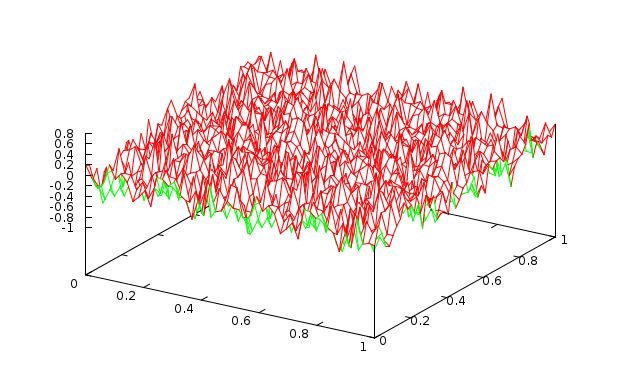
\includegraphics[width=0.3\textwidth]{images/1level_1jac09.png}}\hspace{0.03\textwidth}
\subfigure[1 level with 10 Jacobi sweeps ($\omega=0.9$)\label{fig:2dlap1110}]{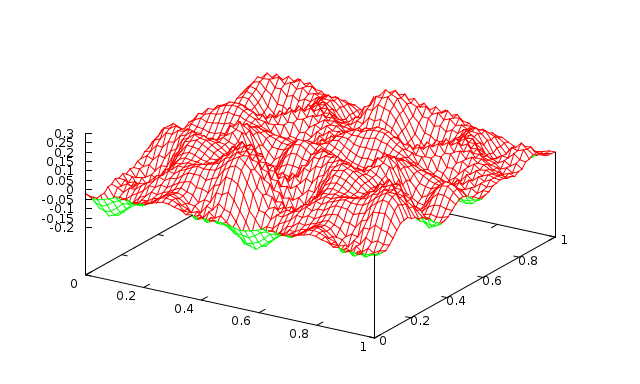
\includegraphics[width=0.3\textwidth]{images/1level_10jac09.png}}\hspace{0.03\textwidth}
\subfigure[1 level with 100 Jacobi sweeps ($\omega=0.9$)\label{fig:2dlap11100}]{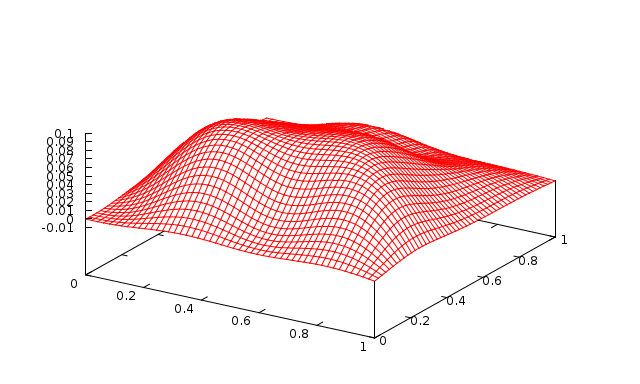
\includegraphics[width=0.3\textwidth]{images/1level_100jac09.png}} \\
\subfigure[2 level with 1 Jacobi sweep ($\omega=0.9$)\label{fig:2dlap121}]{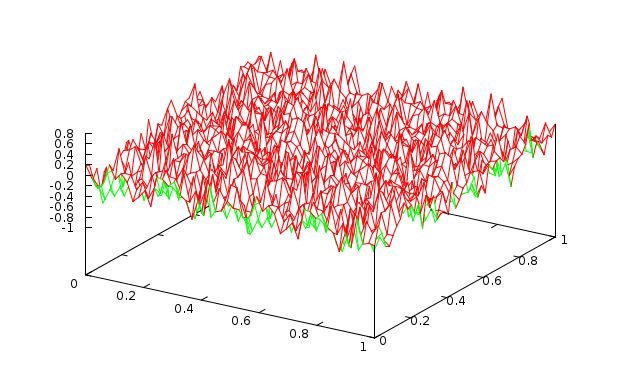
\includegraphics[width=0.3\textwidth]{images/2level_1jac09.png}}\hspace{0.03\textwidth}
\subfigure[2 level with 10 Jacobi sweeps ($\omega=0.9$)\label{fig:2dlap1210}]{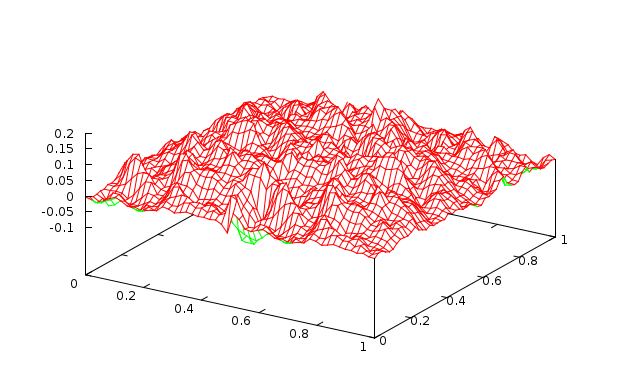
\includegraphics[width=0.3\textwidth]{images/2level_10jac09.png}}\hspace{0.03\textwidth}
\subfigure[2 level with 100 Jacobi sweeps ($\omega=0.9$)\label{fig:2dlap12100}]{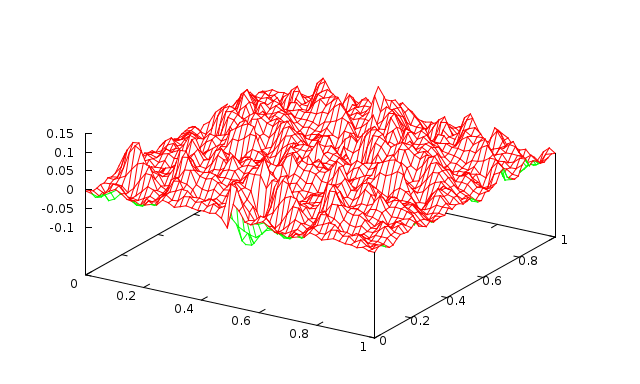
\includegraphics[width=0.3\textwidth]{images/2level_100jac09.png}} \\
\subfigure[3 level with 1 Jacobi sweep ($\omega=0.9$)\label{fig:2dlap131}]{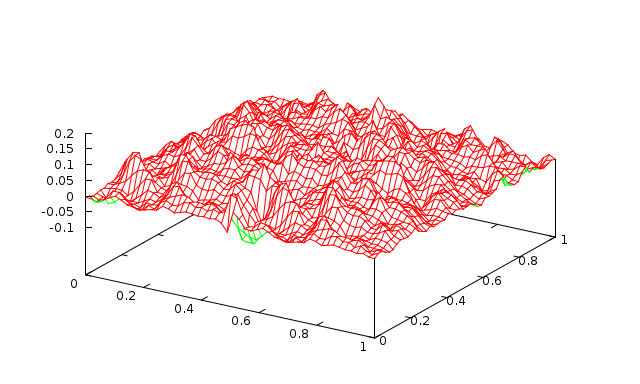
\includegraphics[width=0.3\textwidth]{images/3level_1jac09.png}}\hspace{0.03\textwidth}
\subfigure[3 level with 10 Jacobi sweeps ($\omega=0.9$)\label{fig:2dlap1310}]{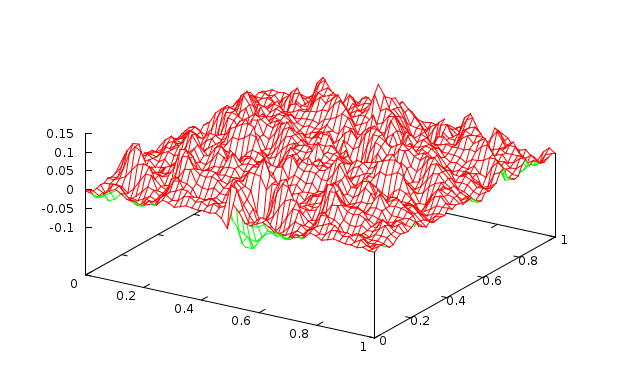
\includegraphics[width=0.3\textwidth]{images/3level_10jac09.png}}\hspace{0.03\textwidth}
\subfigure[3 level with 100 Jacobi sweeps ($\omega=0.9$)\label{fig:2dlap13100}]{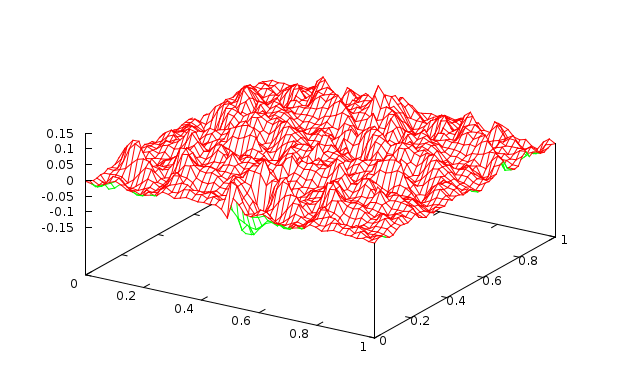
\includegraphics[width=0.3\textwidth]{images/3level_100jac09.png}} \\
\caption{2D Laplace equation on $50\times 50$ mesh after 1 V-cycle with an AMG multigrid solver and Jacobi smoothers on all multigrid levels. (2 processors)}
\end{figure}


\begin{figure}
\subfigure[1 level with 1 Jacobi sweep ($\omega=0.9$)\label{fig:2dlap511}]{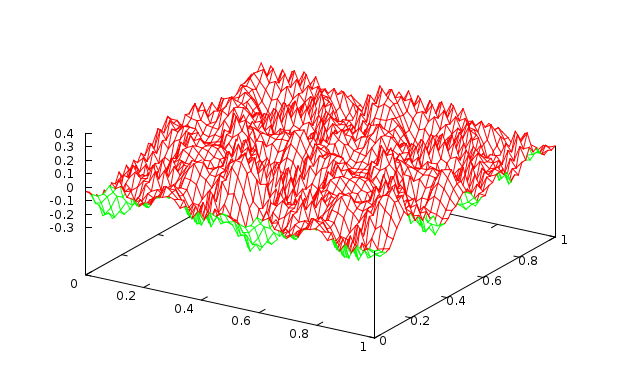
\includegraphics[width=0.3\textwidth]{images/5sweeps_1level_1jac09.png}}\hspace{0.03\textwidth}
\subfigure[1 level with 10 Jacobi sweeps ($\omega=0.9$)\label{fig:2dlap5110}]{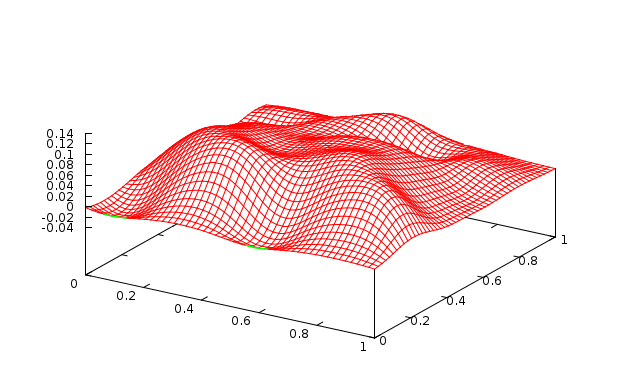
\includegraphics[width=0.3\textwidth]{images/5sweeps_1level_10jac09.png}}\hspace{0.03\textwidth}
\subfigure[1 level with 100 Jacobi sweeps ($\omega=0.9$)\label{fig:2dlap51100}]{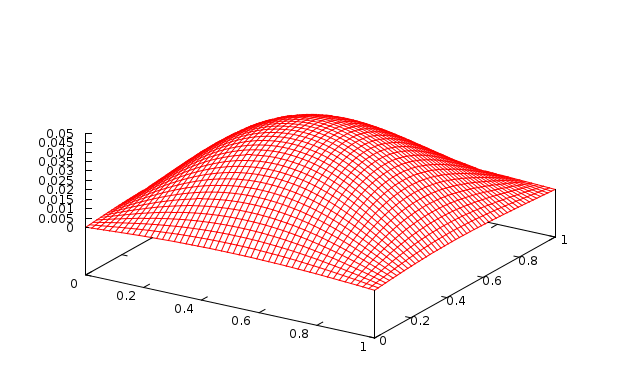
\includegraphics[width=0.3\textwidth]{images/5sweeps_1level_100jac09.png}} \\
\subfigure[2 level with 1 Jacobi sweep ($\omega=0.9$)\label{fig:2dlap521}]{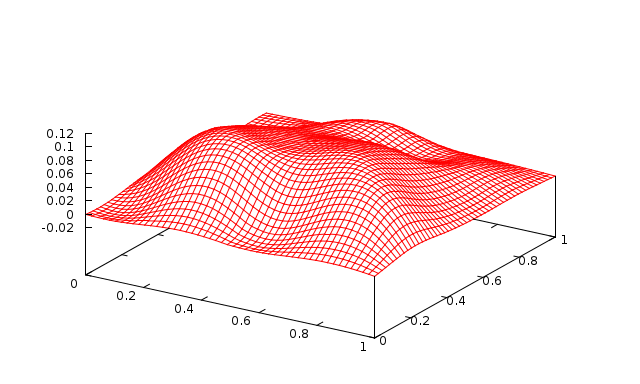
\includegraphics[width=0.3\textwidth]{images/5sweeps_2level_1jac09.png}}\hspace{0.03\textwidth}
\subfigure[2 level with 10 Jacobi sweeps ($\omega=0.9$)\label{fig:2dlap5210}]{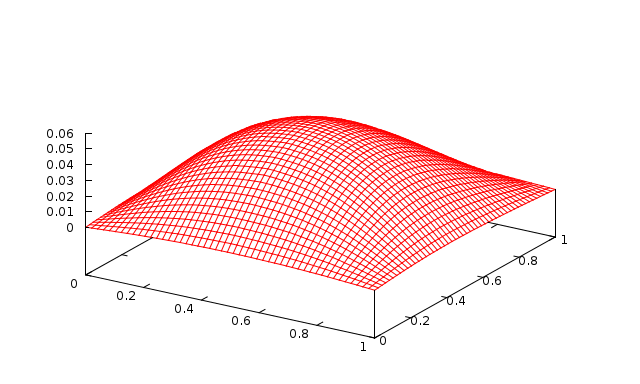
\includegraphics[width=0.3\textwidth]{images/5sweeps_2level_10jac09.png}}\hspace{0.03\textwidth}
\subfigure[2 level with 100 Jacobi sweeps ($\omega=0.9$)\label{fig:2dlap52100}]{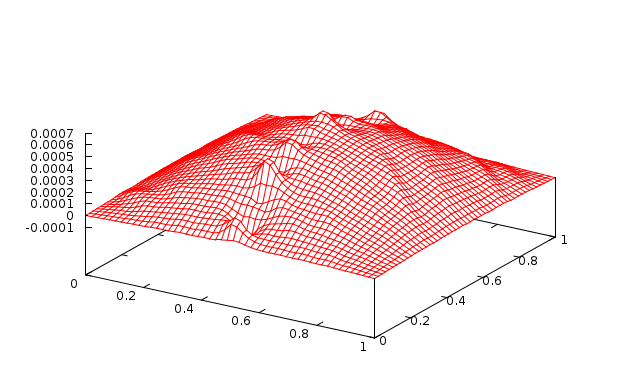
\includegraphics[width=0.3\textwidth]{images/5sweeps_2level_100jac09.png}} \\
\subfigure[3 level with 1 Jacobi sweep ($\omega=0.9$)\label{fig:2dlap531}]{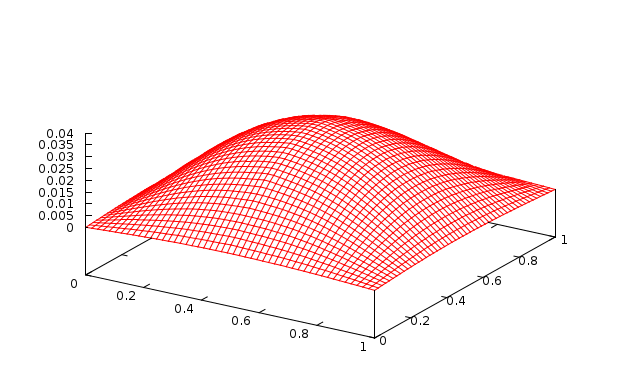
\includegraphics[width=0.3\textwidth]{images/5sweeps_3level_1jac09.png}}\hspace{0.03\textwidth}
\subfigure[3 level with 10 Jacobi sweeps ($\omega=0.9$)\label{fig:2dlap5310}]{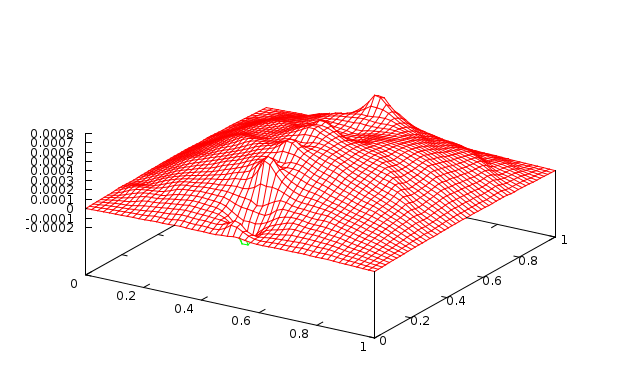
\includegraphics[width=0.3\textwidth]{images/5sweeps_3level_10jac09.png}}\hspace{0.03\textwidth}
\subfigure[3 level with 100 Jacobi sweeps ($\omega=0.9$)\label{fig:2dlap53100}]{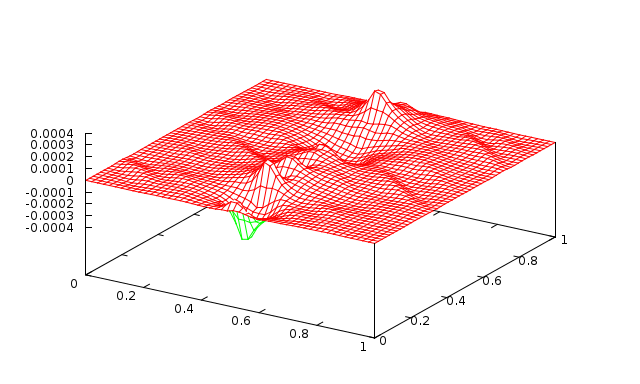
\includegraphics[width=0.3\textwidth]{images/5sweeps_3level_100jac09.png}} \\
\caption{2D Laplace equation on $50\times 50$ mesh after 5 V-cycle with an AMG multigrid solver and Jacobi smoothers on all multigrid levels. (2 processors)}
\end{figure}

\paragraph{Step 4: Use better level smoothers.}
The Jacobi iteration might be a very cheap and fully parallel level smoother, but often one obtains better results when using more expensive and better level smoothers.
In the example XML files there are sections for many possible level smoothers, such that polynomial smoothers (Chebyshev) as well as Gauss-Seidel variants. Usually a small number of smoothing sweeps (e.g. 1 - 5) is sufficient for smoothing the high frequency error without too high costs. More challenging is to find a proper choice for the damping parameters which are highly problem dependent.

\begin{graybox}
 \textbf{Exercise}
 \begin{itemize}
  \item In the xml paramter file \verb|xml/s2b.xml| you can find the definition of some other types of multigrid level smoothers, such as Chebyshev, Jacobi and different Gauss-Seidel variants.
  \item Run the \verb|hands-on.sh| script for the 2D Laplace example and use the \verb|xml/s2b.xml| solver file. Change the \verb|Smoother| parameter in the \verb|AllButCoarsestLevel| section from \verb|myJacobi| to some other smoother that is defined in the \verb|Factories| section, e.g. \verb|SymGaussSeidel|.
  \item Play around with different level smoothers and smoother parameters.
 \end{itemize}
\end{graybox}


\section{Tutorial 3}

\subsection{Test example}
The \texttt{Recirc2D} example uses a matrix corresponding to the finite-difference discretization of the problem
\begin{displaymath}
-\varepsilon\Delta u + (v_x,v_y)\cdot \nabla u=f
\end{displaymath}
on the unit square, with $\varepsilon=1e-5$ and homogeneous Dirichlet boundary conditions. It is $v_x=4x(x-1)(1-2y)$ and $v_y=-4y(y-1)(1-2x)$.
The right hand side vector $f$ is chosen to be the constant vector 1. Due to the convective term the resulting linear system is non-symmetric and therefore more challenging for the iterative solver. The multigrid algorithm has to be adapted to the non-symmetry to obtain good convergence behaviour.

%\subsection{Test program}

\subsection{Multigrid setup phase}

Smoothed aggregation based algebraic multigrid methods originally have not been designed for non-symmetric linear systems. Inappropriately smoothed transfer operators may significantly detoriate the convergence rate or even break convergence completely. 

\paragraph{Non-smoothed transfer operators.}
Before we introduce smoothed aggregation methods for non-symmetric linear systems we first go back one step and demonstrate how to use non-smoothed transfer operators which are eligible for non-symmetric linear systems. Figure \ref{fig:simpledesignnonsmoothed} gives a simplified example how to build the coarse level matrix $A_c$ using the fine level matrix $A$ only. First, we "somehow" build aggregates using the information of the fine level matrix $A$. The aggregates are then used to build the tentative non-smoothed prolongation operator. The restrictor is just the transpose of the (tentative) prolongator and finally the coarse level matrix $A_c$ is calculated by the triple product $A_c=RAP$.

In figure \ref{fig:simpledesignsaamg} the \verb|SaPFactory| has been added after the \verb|TentativePFactory|. Therein the non-smoothed transfer operator from the \verb|TentativePFactory| is smoothed using information of the fine level matrix $A$. This transfer operator design is used per default when the user does not specify its own transfer operator design. The default settings are optimal for symmetric positive definite systems. However for our non-symmetric problem they might be problematic.

\begin{figure}
\subfigure[Non-smoothed aggregation based AMG\label{fig:simpledesignnonsmoothed}]{
\scalebox{0.5}{
\begin{tikzpicture}[>=latex',font={\sf \small}, node distance=2cm]
\def\datawidth{2cm}
\def\dataheight{0.5cm}
\def\factorywidth{4cm}
\def\factoryheight{0.75cm}
%\draw[help lines] (-10,-10) grid (10,10);
\begin{scope}[>=triangle 60]
\node(A) at (-3,10) [draw, terminal, minimum width=\datawidth, minimum height=\dataheight]{$A$};
\node(nothing) at (-3,8) [draw, process, minimum width=\factorywidth, minimum height=\factoryheight]{...};
\node [draw, process, minimum width=\factorywidth, minimum height=\factoryheight, below of=nothing] (AggregationFactory) {AggregationFactory};
\node [draw, process, minimum width=\factorywidth, minimum height=\factoryheight, below of=AggregationFactory] (TentativePFactory) {TentativePFactory};
\node [draw, process, minimum width=\factorywidth, minimum height=\factoryheight, right of=TentativePFactory,node distance=6cm] (TransPFactory) {TransPFactory};
\node [draw, process, minimum width=\factorywidth, minimum height=\factoryheight, below of=TentativePFactory] (RAPFactory) {RAPFactory};
\node(A2) at (-3,0) [draw, terminal, minimum width=\datawidth, minimum height=\dataheight]{$A_c$};
\draw[->] (A) -- (nothing);
\draw[->] (nothing) -- (AggregationFactory);
\draw[->] (A) to[out=180,in=180] node [near start, left] {} (TentativePFactory);
\draw[->] (A) to[out=180,in=180] node [near start, left] {} (RAPFactory);
\draw[->] (AggregationFactory) -- node [near start, left] {Aggregates} (TentativePFactory);
\draw[->] (TentativePFactory) -- node [near start, below] {P} (TransPFactory);
\draw[->] (TentativePFactory) -- node [near start, left] {P} (RAPFactory);
\draw[->] (TransPFactory) -- node [near start, below] {R} (RAPFactory);
\draw[->] (RAPFactory) -- node [near start, below] {} (A2);
\end{scope}
\end{tikzpicture}
} % end scalebox
} % end subfigure 1
\subfigure[Smoothed aggregation AMG (SA-AMG)\label{fig:simpledesignsaamg}]{
\scalebox{0.5}{
\begin{tikzpicture}[>=latex',font={\sf \small}, node distance=2cm]
\def\datawidth{2cm}
\def\dataheight{0.5cm}
\def\factorywidth{4cm}
\def\factoryheight{0.75cm}
%\draw[help lines] (-10,-10) grid (10,10);
\begin{scope}[>=triangle 60]
\node(A) at (-3,10) [draw, terminal, minimum width=\datawidth, minimum height=\dataheight]{$A$};
\node(nothing) at (-3,8) [draw, process, minimum width=\factorywidth, minimum height=\factoryheight]{...};
\node [draw, process, minimum width=\factorywidth, minimum height=\factoryheight, below of=nothing] (AggregationFactory) {AggregationFactory};
\node [draw, process, minimum width=\factorywidth, minimum height=\factoryheight, below of=AggregationFactory] (TentativePFactory) {TentativePFactory};
\node [draw, process, minimum width=\factorywidth, minimum height=\factoryheight, below of=TentativePFactory] (SaPFactory) {SaPFactory};
\node [draw, process, minimum width=\factorywidth, minimum height=\factoryheight, right of=SaPFactory,node distance=6cm] (TransPFactory) {TransPFactory};
\node [draw, process, minimum width=\factorywidth, minimum height=\factoryheight, below of=SaPFactory] (RAPFactory) {RAPFactory};
\node(A2) at (-3,-2) [draw, terminal, minimum width=\datawidth, minimum height=\dataheight]{$A_c$};
\draw[->] (A) -- (nothing);
\draw[->] (nothing) -- (AggregationFactory);
\draw[->] (A) to[out=180,in=180] node [near start, left] {} (TentativePFactory);
\draw[->] (A) to[out=180,in=180] node [near start, left] {} (SaPFactory);
\draw[->] (A) to[out=180,in=180] node [near start, left] {} (RAPFactory);
\draw[->] (AggregationFactory) -- node [near start, left] {Aggregates} (TentativePFactory);
\draw[->] (TentativePFactory) -- node [near start, left] {P} (SaPFactory);
\draw[->] (SaPFactory) -- node [near start, below] {P} (TransPFactory);
\draw[->] (SaPFactory) -- node [near start, left] {P} (RAPFactory);
\draw[->] (TransPFactory) -- node [near start, below] {R} (RAPFactory);
\draw[->] (RAPFactory) -- node [near start, below] {} (A2);
\end{scope}
\end{tikzpicture}
} % end scalebox
} % end subfigure 2
\caption{Simple factory design for aggregation based algebraic multigrid methods.}
\label{fig:simpledesign}
\end{figure}

\paragraph{Smoothed transfer operators for non-symmetric systems.}
In case of non-symmetric linear systems it is $A\neq A^T$. Therefore it is a bad idea just to use the transposed of the smoothed prolongation operator for the restrictor. Let $\widehat{P}$ be the non-smoothed tentative prolongation operator. Then the smoothed prolongation operator $P$ is built using
\begin{displaymath}
P = \bigl(I-\omega A\bigr) \widehat{P},
\end{displaymath}
with some reasonable smoothing parameter $\omega>0$.
The standard restrictor is 
\begin{displaymath}
R = P^T = \widehat{P}^T - \omega \widehat{P}^T A^T = \widehat{P}^T\bigl(I-\omega A^T\bigr).
\end{displaymath}
That is, the restrictor would be smoothed using the information of $A^T$. However, for non-symmetric systems we want to use the information of matrix $A$ for smoothing the restriction operator, too. The restriction operator shall we built by the formula
\begin{displaymath}
R = P^T = \widehat{P}^T - \omega \widehat{P}^T A.
\end{displaymath}
This corresponds to apply the same smoothing strategy to the non-smoothed restriction operator $\widehat{R}=\widehat{P}^T$ which is applied to the (tentative) prolongation operator with using $A^T$ as input instead of matrix $A$. Figure \ref{fig:simpledesignpgamg} shows the changed factory design. The dashed line denotes, that the same smoothing strategy is used than for the prolongation operator. The concept is known as Petrov-Galerkin smoothed aggregation approach in the literature.
A more advanced transfer operator smoothing strategy for non-symmetric linear systems that is based on the Petrov-Galerkin approach is described in \cite{sala2008}. Another approach based on SchurComplement approximations can be found in \cite{wiesner2013}.

\begin{figure}
\scalebox{0.5}{
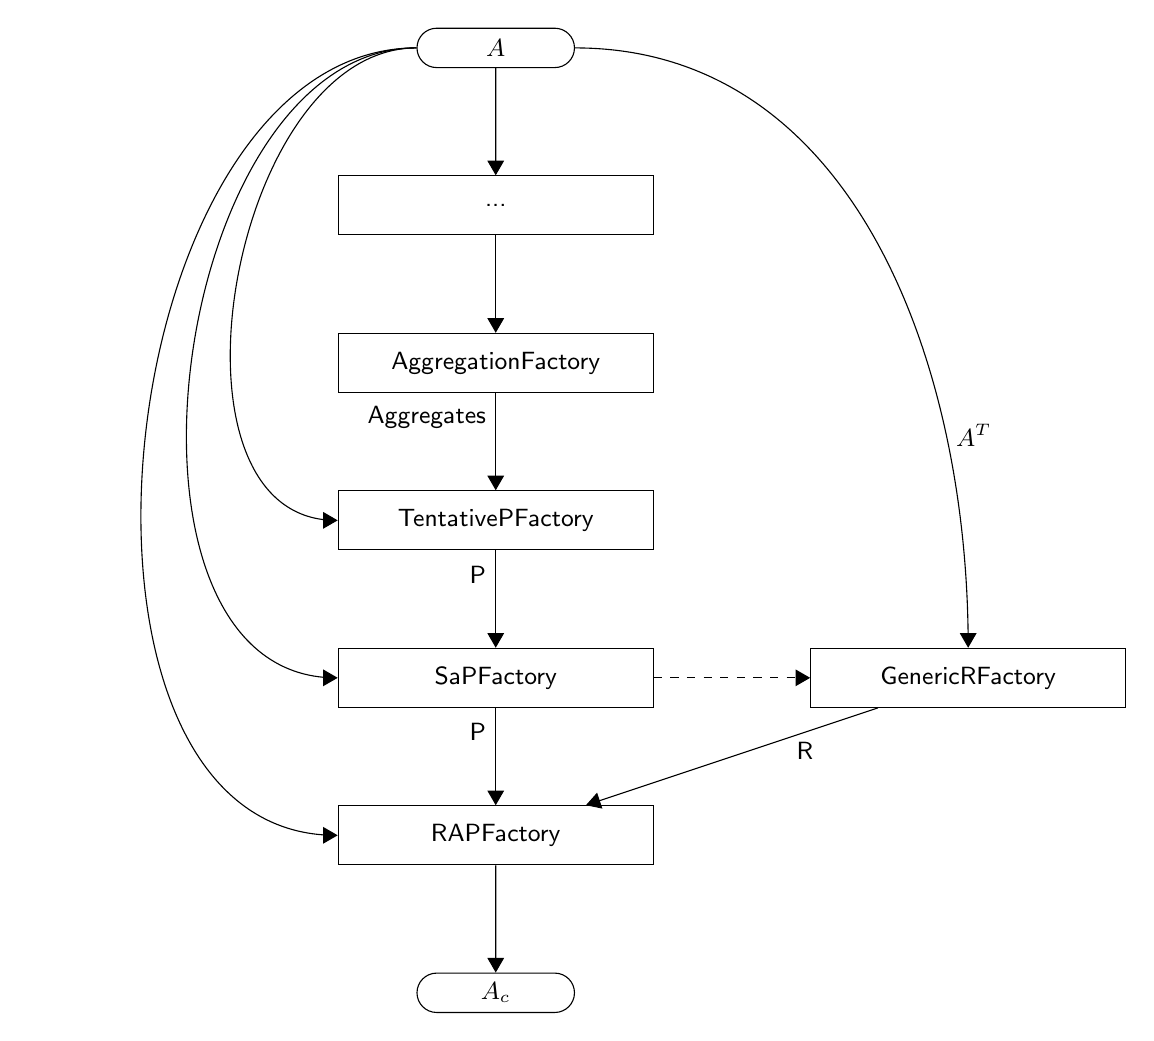
\begin{tikzpicture}[>=latex',font={\sf \small}, node distance=2cm]
\def\datawidth{2cm}
\def\dataheight{0.5cm}
\def\factorywidth{4cm}
\def\factoryheight{0.75cm}
%\draw[help lines] (-10,-10) grid (10,10);
\begin{scope}[>=triangle 60]
\node(A) at (-3,10) [draw, terminal, minimum width=\datawidth, minimum height=\dataheight]{$A$};
\node(nothing) at (-3,8) [draw, process, minimum width=\factorywidth, minimum height=\factoryheight]{...};
\node [draw, process, minimum width=\factorywidth, minimum height=\factoryheight, below of=nothing] (AggregationFactory) {AggregationFactory};
\node [draw, process, minimum width=\factorywidth, minimum height=\factoryheight, below of=AggregationFactory] (TentativePFactory) {TentativePFactory};
\node [draw, process, minimum width=\factorywidth, minimum height=\factoryheight, below of=TentativePFactory] (SaPFactory) {SaPFactory};
\node [draw, process, minimum width=\factorywidth, minimum height=\factoryheight, right of=SaPFactory,node distance=6cm] (GenericRFactory) {GenericRFactory};
\node [draw, process, minimum width=\factorywidth, minimum height=\factoryheight, below of=SaPFactory] (RAPFactory) {RAPFactory};
\node(A2) at (-3,-2) [draw, terminal, minimum width=\datawidth, minimum height=\dataheight]{$A_c$};
\draw[->] (A) -- (nothing);
\draw[->] (nothing) -- (AggregationFactory);
\draw[->] (A) to[out=180,in=180] node [near start, left] {} (TentativePFactory);
\draw[->] (A) to[out=180,in=180] node [near start, left] {} (SaPFactory);
\draw[->] (A) to[out=180,in=180] node [near start, left] {} (RAPFactory);
\draw[->] (A) to[out=0,in=90] node [near end, right] {$A^T$} (GenericRFactory);
\draw[->] (AggregationFactory) -- node [near start, left] {Aggregates} (TentativePFactory);
\draw[->] (TentativePFactory) -- node [near start, left] {P} (SaPFactory);
\draw[->,dashed] (SaPFactory) -- node [near start, below] {} (GenericRFactory);
\draw[->] (SaPFactory) -- node [near start, left] {P} (RAPFactory);
\draw[->] (GenericRFactory) -- node [near start, below] {R} (RAPFactory);
\draw[->] (RAPFactory) -- node [near start, below] {} (A2);
\end{scope}
\end{tikzpicture}
} % end scalebox
\caption{Simple factory design for smoothed aggregation based algebraic multigrid methods for non-symmetric systems.}
\label{fig:simpledesignpgamg}
\end{figure}



\subsection{XML Interface}

\paragraph{Non-smoothed transfer operators}

Listing \ref{listing:PAAMGXML} shows the parameters for non-smoothed transfer operators. 

The aggregates are built by the \verb|UncoupledAggregationFactory| which means that aggregates cannot overlap processor boundaries.

\begin{Listing} 
\begin{center} 
\begin{lstlisting}[language=XML,label=listing:PAXML]
<ParameterList name="MueLu">
  <!-- Factory collection -->
  <ParameterList name="Factories">
    <ParameterList name="UncoupledAggregationFact">
      <Parameter name="factory" type="string" value="UncoupledAggregationFactory"/>
      <Parameter name="Ordering" type="string" value="Natural"/>
      <Parameter name="MinNodesPerAggregate" type="int" value="4"/>
    </ParameterList>   
    <ParameterList name="myTentativePFact">
     <Parameter name="factory" type="string" value="TentativePFactory"/>
    </ParameterList>
    <ParameterList name="myRestrictorFact">
     <Parameter name="factory" type="string" value="TransPFactory"/>
     <Parameter name="P" type="string" value="myTentativePFact"/>
    </ParameterList>
  </ParameterList>

  <!-- Definition of the multigrid preconditioner -->
  <ParameterList name="Hierarchy">
    <Parameter name="numDesiredLevel" type="int" value="10"/>
    <Parameter name="maxCoarseSize" type="int" value="10"/>
    <Parameter name="verbosity" type="string" value="High"/>
    <ParameterList name="All">
      <Parameter name="Aggregates" type="string"   value="UncoupledAggregationFact"/>
      <Parameter name="Nullspace" type="string"   value="myTentativePFact"/>
      <Parameter name="P" type="string"   value="myTentativePFact"/>
      <Parameter name="R" type="string"   value="myRestrictorFact"/>
      <Parameter name="CoarseSolver" type="string"   value="DirectSolver"/>
    </ParameterList>
  </ParameterList>
</ParameterList>
\end{lstlisting}
\caption{Structure of XML input file for \MueLu~ with non-smoothed aggregation transfer operators.} 
\label{listing:PAAMGXML}
\end{center}
\end{Listing}

In figure \ref{fig:ucoutput} a typical output (verbosity level "High") for \MueLu~ with uncoupled aggregation and non-smoothed transfer operators is shown as it is defined in the parameter list in listing \ref{listing:PAAMGXML} and shown in figure \ref{fig:simpledesignnonsmoothed}.
\begin{figure}
\tiny
\begin{verbatim}
 Build (MueLu::TentativePFactory)
  Build (MueLu::UncoupledAggregationFactory)
   Build (MueLu::CoalesceDropFactory)
    lightweight wrap = 0
    CoalesceDropFactory::Build(): found blockdim=1 from strided maps. offset=0
    Build (MueLu::AmalgamationFactory)
     AmalagamationFactory::Build(): found fullblocksize=1 and stridedblocksize=1 from strided maps. offset=0
    CoalesceDropFactory::SetupAmalgamationData() # of amalgamated blocks=2500
    CoalesceDropFactory: nodeMap 1250/2500 elements
   BuildAggregates (MueLu::OnePtAggregationAlgorithm)
    Aggregation (UC): Phase 0 (1pt aggregates): Nodes aggregated = 0 out of 2500 nodes
    Aggregation (UC): Phase 0 (1pt aggregates): Total aggregates = 0
    Aggregation (UC): Phase 0 (1pt aggregates): (WARNING) 2500 unaggregated nodes left
   BuildAggregates (MueLu::UncoupledAggregationAlgorithm)
    Aggregation (UC): UncoupledAggregationAlgorithm: Nodes aggregated = 2116 out of 2500 nodes
    Aggregation (UC): UncoupledAggregationAlgorithm: Total aggregates = 442
    Aggregation (UC): UncoupledAggregationAlgorithm: (WARNING) 384 unaggregated nodes left
   BuildAggregates (MueLu::MaxLinkAggregationAlgorithm)
    Aggregation (UC): Phase 2 (max_link, extend aggregates): Nodes aggregated = 2500 out of 2500 nodes
    Aggregation (UC): Phase 2 (max_link, extend aggregates): Total aggregates = 442
   BuildAggregates (MueLu::IsolatedNodeAggregationAlgorithm)
    Aggregation (UC): Phase 4 (isolated node aggregation): Nodes aggregated = 2500 out of 2500 nodes
    Aggregation (UC): Phase 4 (isolated node aggregation): Total aggregates = 442
   BuildAggregates (MueLu::EmergencyAggregationAlgorithm)
    Aggregation (UC): Phase 3 (emergency aggregation): Nodes aggregated = 2500 out of 2500 nodes
    Aggregation (UC): Phase 3 (emergency aggregation): Total aggregates = 442
   "UC": MueLu::Aggregates{nGlobalAggregates = 442}
  Build (MueLu::CoarseMapFactory)
   domainGIDOffset: 0 block size: 1 stridedBlockId: -1
  TentativePFactory : aggregates do not cross process boundaries
  Ptent size =  2500 x 442, nnz = 2500
  Ptent Load balancing info:
  Ptent   # active processes: 2,  # processes with data = 2
  Ptent   # rows per proc   : avg = 1.25e+03,  dev =  0.0%,  min =  +0.0%,  max =  +0.0%
  Ptent   #  nnz per proc   : avg = 1.25e+03,  dev =  0.0%,  min =  +0.0%,  max =  +0.0%
 Transpose P (MueLu::TransPFactory)
 Computing Ac (MueLu::RAPFactory)
  MxM: A x P
   ****** USING ML's MATRIX MATRIX MULTIPLY (LNM version) ******
  MxM: R x (AP) (explicit)
   ****** USING ML's MATRIX MATRIX MULTIPLY (LNM version) ******
  Ac size =  442 x 442, nnz = 2892
  Ac Load balancing info:
  Ac   # active processes: 2,  # processes with data = 2
  Ac   # rows per proc   : avg = 2.21e+02,  dev =  0.0%,  min =  +0.0%,  max =  +0.0%
  Ac   #  nnz per proc   : avg = 1.45e+03,  dev =  0.0%,  min =  +0.0%,  max =  +0.0%
\end{verbatim}
\caption{Exemplary output of \MueLu~ when generating the coarse level matrix $A_c$ using non-smoothed prolongation and restriction operators and uncoupled aggregation.}
\label{fig:ucoutput}
\end{figure}

\begin{graybox}
 \textbf{Exercise}
 \begin{itemize}
  \item Run the \verb|hands-on.sh| script for the 2D Recirc example and use the \verb|xml/s3a.xml| solver file. The \verb|xml/s3a.xml| contains non-smoothed transfer operators, a Jacobi smoother and a symmetric GaussSeidel smoother. Find reasonable smoother settings.
  \item Try different values for the \verb|MinNodesPerAggregate| parameter. The parameter defines the minimum size of nodes of each aggregate. How does the multigrid setup differ when using a small value (e.g. 3), a value in the medium range (e.g. 6) and a big value (e.g. 12)?
 \end{itemize}
\end{graybox}

Choosing \verb|MinNodesPerAggregate|$=4$ we obtain a 4 level multigrid method:
{\footnotesize
\begin{verbatim}
 --------------------------------------------------------------------------------
 ---                            Multigrid Summary                             ---
 --------------------------------------------------------------------------------
 Number of levels    = 4
 Operator complexity = 1.27
 Max Coarse Size     = 10
 Implicit Transpose  = false
 
 matrix rows    nnz  nnz/row procs
 A 0    2500  12300     4.92  2
 A 1     442   2892     6.54  2
 A 2      60    348     5.80  2
 A 3      10     46     4.60  2
\end{verbatim}}

When using \verb|MinNodesPerAggregate|$=9$ the multigrid setup routine produces a 6 level multigrid method
{\footnotesize
\begin{verbatim}
 --------------------------------------------------------------------------------
 ---                            Multigrid Summary                             ---
 --------------------------------------------------------------------------------
 Number of levels    = 6
 Operator complexity = 1.92
 Max Coarse Size     = 10
 Implicit Transpose  = false
 
 matrix rows    nnz  nnz/row procs
 A 0    2500  12300     4.92  2
 A 1    1250   8450     6.76  2
 A 2     326   2128     6.53  2
 A 3      92    562     6.11  2
 A 4      28    160     5.71  2
 A 5       8     34     4.25  2
\end{verbatim}}

When using even bigger numbers for \verb|MinNodesPerAggregate| the results should not change. A closer look to the output of the aggregation factory reveals that the aggregation factory was not able to build aggregates as big as the user desired. The aggregation algorithm then builds small "emergency" aggregates. It's important to choose a reasonable value for the minimum size of the aggregates to obtain a good coarsening rate and a low operator complexity. The idea of the \verb|MinNodesPerAggregate| is to define a desired coarsening ratio, but be aware, that it cannot guarantee a high coarsening rate if this parameter is chosen too high.

\paragraph{Smoothed aggregation for non-symmetric problems}
Next, let's try smoothed transfer operators for the non-symmetric linear system and compare the results of the transfer operator designs in \ref{fig:simpledesignsaamg} and \ref{fig:simpledesignpgamg} with the non-smoothed transfer operators.

\begin{Listing}
\begin{center}
\begin{lstlisting}[language=xml]
<ParameterList name="myTentativePFact">
 <Parameter name="factory" type="string" value="TentativePFactory"/>
</ParameterList>
<ParameterList name="myProlongatorFact">
 <Parameter name="factory" type="string" value="SaPFactory"/>
 <!--<Parameter name="factory" type="string" value="PgPFactory"/>-->
 <Parameter name="P" type="string" value="myTentativePFact"/>
</ParameterList>
<ParameterList name="myRestrictorFact">
 <Parameter name="factory" type="string" value="TransPFactory"/>
 <Parameter name="P" type="string" value="myProlongatorFact"/>
 <!--<Parameter name="P" type="string" value="myTentativePFact"/>-->
 <!--<Parameter name="factory" type="string" value="GenericRFactory"/>-->
</ParameterList>
\end{lstlisting}
\caption{Fragment of XML input file for different transfer operators.} 
\label{listing:Transfers}
\end{center}
\end{Listing}

In listing \ref{listing:Transfers} one can find some fragments of the XML parameters for the transfer operators. Note, that some options are commented out and inactive (using the \verb|<!--  -->| keywords).

\begin{graybox}
 \textbf{Exercise}
 \begin{itemize}
  \item Load the \verb|Recirc2D| example on a $50\times 50$ mesh. Create your own \verb|mysolvers.xml| XML parameter file using the \verb|xml/s3b.xml| file as template. It contains the standard parameters including the definitions of listing \ref{listing:Transfers}. Run the example with your \verb|mysolvers.xml| file as solver input.
  \item The parameters from \verb|xml/s3b.xml| define the standard smoothed aggregation transfer operators for symmetric problems. Compare the output with the non-smoothed transfer operators from \verb|xml/s3a.xml|. How do the different transfer operator strategies affect the convergence behaviour and the number of GMRES iterations?
  \item Change the factory for the restriction operator from \verb|TransPFactory| to \verb|GenericRFactory| and rerun the example. How do the results change?
  \item Change the prolongation smoothing strategy from \verb|SaPFactory| to \verb|PgPFactory|. How do the results change?
  \item Try to use a smoothed prolongation operator with a non-smoothed restriction operator. How does it affect the results? Important: the \verb|GenericRFactory| does not accept a tentative prolongation operator as input. Use the \verb|TransPFactory| as base for the restriction operator with the tentative prolongator as input!
 \end{itemize}
\end{graybox}

Solving the \texttt{Recirc2D} example on the $50\times 50$ mesh with the default solver parameters from \verb|xml/s3a.xml| needs 19 GMRES iterations with the 4 level AMG preconditioner. When using smoothed aggregation as in \ref{fig:simpledesignsaamg} (default settings from \verb|xml/s3b.xml|) 29 GMRES iterations are needed. Obviously smoothed aggregation (SA-AMG) with the transposed smoothed prolongator as restriction operator is not designed for non-symmetric problems. 

If we keep the \verb|SaPFactory| for smoothing the prolongation operator but change from the \verb|TransPFactory| to the \verb|GenericRFactory| which corresponds to use a Petrov Galerkin approach for transfer operator smoothing we can reduce the number of GMRES iterations to 22 which is still higher than for the non-smoothed transfer operators. If we finally change the prolongation smoothing strategy from the \verb|SaPFactory| to \verb|PgPFactory| and keep the Petrov Galerkin approach for the restriction operators we only need 13 GMRES iterations to solve the problem. These (optimal) settings can be found in \verb|xml/s3c.xml|. In contrary to \verb|SaPFactory| which chooses too high smoothing parameters $\omega$ resulting from some eigenvalue estimations which are only valid for symmetric linear systems, the \verb|PgPFactory| generates variable damping parameters using some energy minimization principles.

\section{Tutorial 4}

\subsection{Building aggregates}

The aggregates are built using the graph of the fine level matrix $A$. The graph is generated by the \verb|CoalesceDropFactory|. Since we still only restrict ourself to scalar problems with one degree of freedom per node (\verb|DofsPerNode|=$1$), the graph of the fine level matrix is trivial to build.
Figure \ref{fig:simpledesignaggregates} shows the extended transfer operator design with the additional \verb|CoalesceDropFactory|.

Especially for anisotropic or non-symmetric problems it may be advantageous to drop small entries from the graph of $A$ and use a filtered graph for generating aggregates. 

In listing \ref{listing:CoalesceDropFactory} one can find the definition of the \verb|myCoalesceDropFactory| which drops all values of the fine level matrix $A$ with the absolute value smaller than $0.01$. Of course, the \verb|myCoalesceDropFactory| has to be registered to generate the variable \verb|Graph|, which is used by the aggregation factory. The user can either define its own aggregation factory (see e.g. previous tutorial) or use the default aggreagtion factory. Be aware that the given XML file is not complete. For demonstration purposes we also introduced a \verb|RAPFactory| which makes use of the user-defined transfer factories \verb|myProlongatorFact| as well as \verb|myRestrictorFact| which are not defined in listing \ref{listing:CoalesceDropFactory}. A full XML file with all necessary definitions can be found in \verb|xml/s4b.xml|.

\begin{figure}
\scalebox{0.6}{
\begin{tikzpicture}[>=latex',font={\sf \small}, node distance=2cm]
\def\datawidth{2cm}
\def\dataheight{0.5cm}
\def\factorywidth{4cm}
\def\factoryheight{0.75cm}
%\draw[help lines] (-10,-10) grid (10,10);
\begin{scope}[>=triangle 60]
\node(A) at (-3,10) [draw, terminal, minimum width=\datawidth, minimum height=\dataheight]{$A$};
\node(CoalesceDropFactory) at (-3,8) [draw, process, minimum width=\factorywidth, minimum height=\factoryheight]{CoalesceDropFactory};
\node [draw, process, minimum width=\factorywidth, minimum height=\factoryheight, below of=nothing] (AggregationFactory) {AggregationFactory};
\node [draw, process, minimum width=\factorywidth, minimum height=\factoryheight, below of=AggregationFactory] (TentativePFactory) {TentativePFactory};
\node [draw, process, minimum width=\factorywidth, minimum height=\factoryheight, below of=TentativePFactory] (SaPFactory) {SaPFactory};
\node [draw, process, minimum width=\factorywidth, minimum height=\factoryheight, right of=SaPFactory,node distance=6cm] (TransPFactory) {TransPFactory};
\node [draw, process, minimum width=\factorywidth, minimum height=\factoryheight, below of=SaPFactory] (RAPFactory) {RAPFactory};
\node [draw, process, minimum width=\factorywidth, minimum height=\factoryheight, right of=RAPFactory,node distance=9cm] (AggExportFactory) {AggregationExportFactory};
\node(A2) at (-3,-2) [draw, terminal, minimum width=\datawidth, minimum height=\dataheight]{$A_c$};
\draw[->] (A) -- (CoalesceDropFactory);
\draw[->] (CoalesceDropFactory) -- node [near start, left] {Graph} (AggregationFactory);
\draw[->] (A) to[out=180,in=180] node [near start, left] {} (TentativePFactory);
\draw[->] (A) to[out=180,in=180] node [near start, left] {} (SaPFactory);
\draw[->] (A) to[out=180,in=180] node [near start, left] {} (RAPFactory);
\draw[->] (AggregationFactory) -- node [near start, left] {Aggregates} (TentativePFactory);
\draw[->] (TentativePFactory) -- node [near start, left] {P} (SaPFactory);
\draw[->] (SaPFactory) -- node [near start, below] {} (TransPFactory);
\draw[->] (SaPFactory) -- node [near start, left] {P} (RAPFactory);
\draw[->] (TransPFactory) -- node [near start, below] {R} (RAPFactory);
\draw[->] (RAPFactory) -- node [near start, below] {} (A2);
\draw[o->] (RAPFactory) -- (AggExportFactory);
\draw[->] (AggregationFactory) to[out=0,in=100] node [near start, right] {Aggregates} (AggExportFactory);
\draw[->] (CoalesceDropFactory) to[out=0,in=80] node [near start, right] {DofsPerNode} (AggExportFactory);
\end{scope}
\end{tikzpicture}
} % end scalebox
\caption{Simple factory design for building aggregates.}
\label{fig:simpledesignaggregates}
\end{figure}

\begin{Listing}
\begin{center}
\begin{lstlisting}[language=xml]
<ParameterList name="Factories">

  <ParameterList name="myCoalesceDropFact">
   <Parameter name="factory" type="string" value="CoalesceDropFactory"/>
   <Parameter name="lightweight wrap" type="bool"   value="true"/>
   <!-- for aggregation dropping -->
   <Parameter name="aggregation threshold" type="double" value="0.01"/>
  </ParameterList>
       
  <ParameterList name="myRAPFact">
   <Parameter name="factory" type="string" value="RAPFactory"/>
   <Parameter name="P" type="string" value="myProlongatorFact"/>
   <Parameter name="R" type="string" value="myRestrictorFact"/>
   <ParameterList name="TransferFactories">
    <!-- <Parameter name="Visualization" type="string" value="myAggExportFact"/> -->
   </ParameterList>
  </ParameterList>  
</ParameterList>

<!-- Definition of the multigrid preconditioner -->
<ParameterList name="Hierarchy">
  <Parameter name="numDesiredLevel" type="int" value="10"/> 
  <Parameter name="maxCoarseSize" type="int" value="10"/>
  <ParameterList name="All">
    <Parameter name="Graph" type="string"   value="myCoalesceDropFact"/>
    <Parameter name="A" type="string"   value="myRAPFact"/>
  </ParameterList>
  ...
</ParameterList>
\end{lstlisting}
\caption{Fragment of XML input file for CoalesceDropFactory with dropping small entries from matrix graph.} 
\label{listing:CoalesceDropFactory}
\end{center}
\end{Listing}

\subsection{Export and visualization of aggregates}
For debugging purposes it can be very useful to visualize the aggregates. In \MueLu~ there is a helper factory named \verb|AggregationExportFactory| which can be used to export the aggregates for visualization purposes. 

The \verb|AggregationExportFactory| acts as a small helper factory within the \verb|RAPFactory| which writes out some aggregation information to files on the hard disk (see figure \ref{fig:simpledesignaggregates}). In a postprocessing step one can use these files together with some mesh information to generate pictures of the aggregates on each level. 

In \verb|xml/s4b.xml| a \verb|AggregationExportFactory| defined and incorporated into the \verb|RAPFactory|. Note, that the export of aggregates is optional. It is necessary to define an \verb|AggregationExportFactory| and a \verb|RAPFactory| for exporting the aggregation information . One cannot use the internal default factories which are automatically generated when not defined by the user explicitely!

\begin{graybox}
 \textbf{Exercise}
 \begin{itemize}
  \item Load the \verb|Laplace2D| example on a $50\times 50$ mesh on 2 processors and apply the \verb|xml/s4a.xml| solver which exports the aggregates. 
  \item Open another terminal and change to the folder with the \verb|hands-on.sh| script. One should find new files with  filenames like \verb|aggs_level0_proc0.txt| which contains the aggregation information for the different multigrid levels and processors. Note, that these files are automatically removed as soon as you finish the \verb|hands-on.sh| script (e.g. using option 11).
  \item Run the \verb|MueLu_Agg2VTK.py| python script which generates some VTK files visualizing the aggregates using the aggregation information and the mesh coordinates. The python script assumes that you have used 2 processors. In case you are using a different number of processors you can adapt the \verb|numprocs| variable in the \verb|MueLu_Agg2VTK.py| script accordingly. Note, the visualization script is not tested for anisotropic meshes.
  \item Use \verb|paraview| to display the \verb|aggs*.vtp| files that have been generated by the postprocessing script \verb|MueLu_Agg2VTK.py|.
 \end{itemize}
\end{graybox}

\begin{graybox}
 \textbf{Exercise}
 \begin{itemize}
  \item Repeat above steps for the \verb|Recirc2D| example on a $50\times 50$ mesh. Compare the aggregates from the \verb|xml/s4a.xml| parameter file with the aggregates when using the \verb|xml/s4b.xml| parameter file, which drops some small entries of the fine level matrix $A$ when building the graph.
  \item Vary the number of processors. Don't forget to adapt the \verb|numprocs| variable in the postprocessing script. In \verb|paraview| choose the variable \verb|proc| for the coloring. Then the color denotes the processor the aggregate belongs to. How do the aggregates change when switching from 2 to 3 processors?
  \item Try the solver parameters from \verb|xml/s4c.xml| vor the \verb|Recirc2D| example on a $50\times 50$ mesh and compare them with the results for the \verb|xml/s4a.xml| and \verb|xml/s4b.xml| parameters. Which differences do you observe?
 \end{itemize}
\end{graybox}

Figure \ref{fig:symAggs} shows the aggregates for the Laplace2D problem on the different multigrid levels starting with an isotropic $50\times 50$ mesh. No dropping of small entries was used when building the matrix graph. For visualization purposes the "midpoint" of each aggregate defines the coordinate of the supernode on the next coarser level. Be aware that these supernodes are purely algebraic. There is no coarse mesh for algebraic multigrid methods. As one can see from the colors an uncoupled aggregation strategy has been applied using 2 processors. The aggregates do not cross the processor boundaries.

\begin{figure}
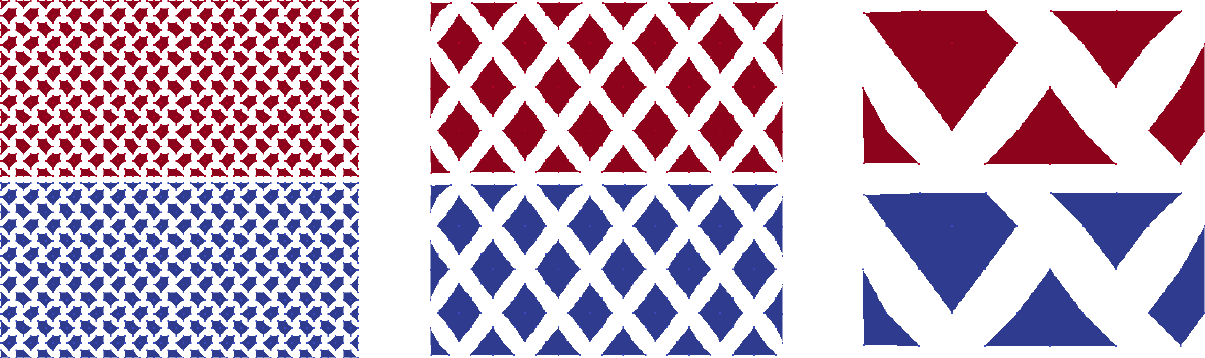
\includegraphics[width=\textwidth]{images/aggsSymm.png} 
\caption{Aggregates for Laplace2D example on $50\times 50$ mesh without dropping.}
\label{fig:symAggs}
\end{figure}

Figure \ref{fig:nonsymAggs} shows the aggregates for the Recirc2D problem. When building the matrix graph, entries with values smaller than $0.01$ were dropped. Obviously the shape of the aggregates follows the direction of convection of the example. Again an uncoupled aggregation strategy has been used on 2 processors. The aggregates do not cross processor boundaries.
\begin{figure}
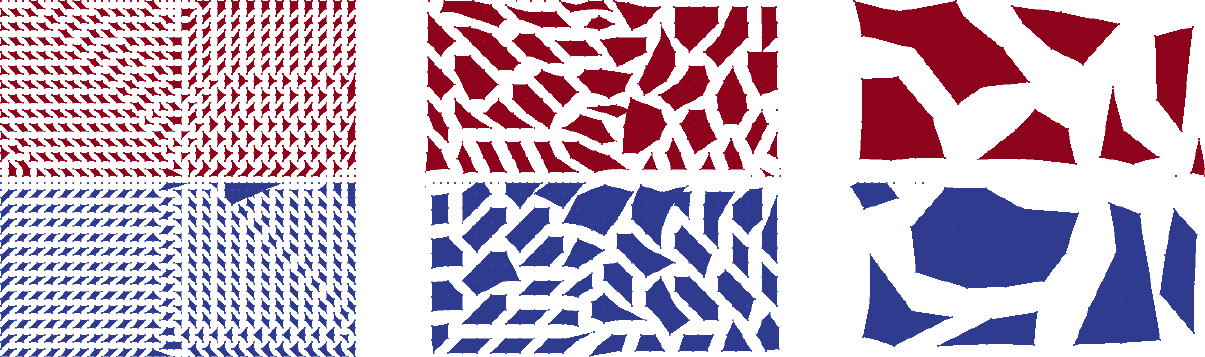
\includegraphics[width=\textwidth]{images/aggsNonSymm.png} 
\caption{Aggregates for Recirc2D example on $50\times 50$ mesh with dropping.}
\label{fig:nonsymAggs}
\end{figure}

Comparing figures ref{fig:symAggs} and \ref{fig:nonsymAggsCoupled} one finds the difference between the \verb|UncoupledAggregationFactory| and the \verb|CoupledAggregationFactory| factory. For the \verb|CoupledAggregationFactory| the aggregates can overlap processor boundaries.
\begin{figure}
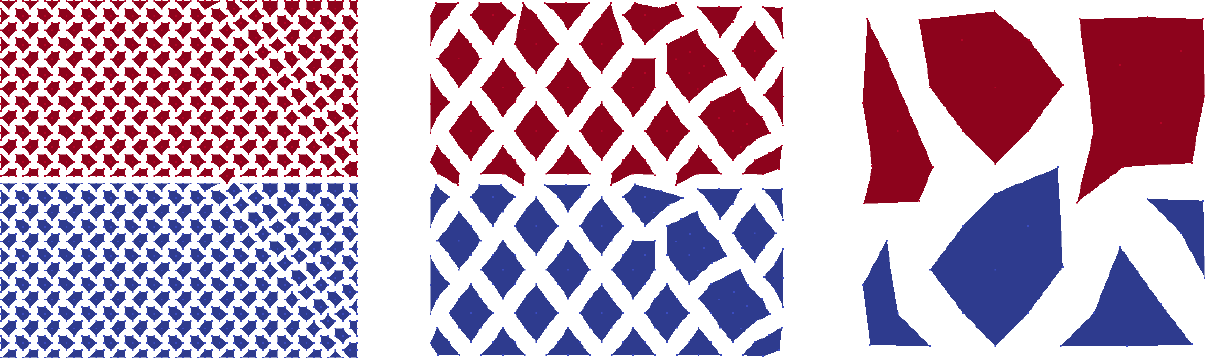
\includegraphics[width=\textwidth]{images/aggsSymmCoupled.png} 
\caption{Aggregates for Laplace2D example on $50\times 50$ mesh without dropping using a coupled aggregation strategy.}
\label{fig:nonsymAggsCoupled}
\end{figure}

Using the \verb|CoupledAggregationFactory| in general is not recommended, since
\begin{itemize}
\item[-] the aggregation routine itself needs some global communication,
\item[-] building the tentative prolongation operator from the aggregates needs some global communication,
\item[-] prolongator smoothing is more expensive due to a higher overlap.
\end{itemize}
The implementation of a \verb|CoupledAggregationFactory| is highly complicated and therefore error-prone and less robust.

\section{Tutorial 5}
\subsection{Rebalancing}
It's a natural thing to use lesser processors for the coarse level problem than for the fine level problem. This is an elegant way to avoid the problems of the coupled aggregation strategy, by just using the uncoupled aggregation strategy with rebalancing on the coarser levels.

In this tutorial we use a hypergraph based repartitioning for the coarse level matrices $A_c$ to rebalance the problem. The repartitioning algorithm is implemented in the Zoltan package of Trilinos. The advantage of the hypergraph based repartitioning methods is, that they do not need additional information such as node coordinates and therefore are the consequent choice within algebraic multigrid preconditioners\footnote{Hypergraph partitioning algorithms as PHG are not available in the new Zoltan2 package of Trilinos. Therefore we can use this type of repartitioning only in context of Epetra based applications. If you use the new templated Tpetra stack you have to use repartitioning algorithms which are available in Zoltan2 such as RCB.}.

Repartitioning algorithms are a very wide field of research and can be very complicated. Here, we cannot go into details and just focus on how to use them. Basically there are only two really important parameters that the user has to set properly:
\begin{description}
\item \textbf{minRowsPerProcessor} the minimum number of rows each processor shall handle. This parameter is used to reduce the number of involved processors on the coarser levels. If for example the parameter value is chosen to be 1000 and the fine level problem has 10000 rows whereas the coarse level problem has 2000 rows, then the fine level problem is solved on not more than 10 processors at maximum and for the coarse level problem there are not more processors than at maximum 2 being used.
\item \textbf{nonzeroImbalance} This parameter defines the maximum allowed imbalance ratio of nonzeros on all processors. If e.g. the value is set to 1.2, and there is one processor with more than 20\% nonzeros compared to another processor, than the problem will be rebalanced.
\end{description}

\subsection{Transfer operator design}

Figure \ref{fig:rebalanceddesignpgamg} gives the extended factory design for smoothed aggregation based AMG for non-symmetric linear systems with rebalancing. Nothing has changed in the upper part where the non-rebalanced Galerkin product has been calculated using the \verb|RAPFactory|. The coarse level matrix $A_c$ as output from the \verb|RAPFactory| then is checked for its partition and rebalanced. 

The \verb|AmalgamationFactory| amalgamates the matrix, i.e. it generates some mapping between the actual degrees of freedom and the corresponding nodes or supernodes. In fact the \verb|AmalgamationFactory| is only important if there are more than one degree of freedom per node. Otherwise the mappings are trivial to build.

The \verb|IsorropiaInterface| class first builds internally the graph of the coarse level matrix $A_c$ using the information from the \verb|AmalgamationInformation| and then calls the repartitioning algorithm from Zoltan through the Isorropia interface\footnote{Isorropia is a Trilinos package which provides an easy-to-use interface to many partitioning algorithms in Zoltan.}. The output is an amalgamated repartitioning information. Then the \verb|RepartitionInterface| factory resembles the un-amalgamated repartitioning information which is put into the \verb|RepartitionFactory|.

The \verb|RepartitionFactory| is the most important factory and responsible for the repartitioning. Therein the decision is made whether repartitioning is necessary at all. It creates the communication "plan" that is used to rebalance the transfer operators and the coarse level matrix.

\begin{figure}
\begin{center}
\scalebox{0.8}{
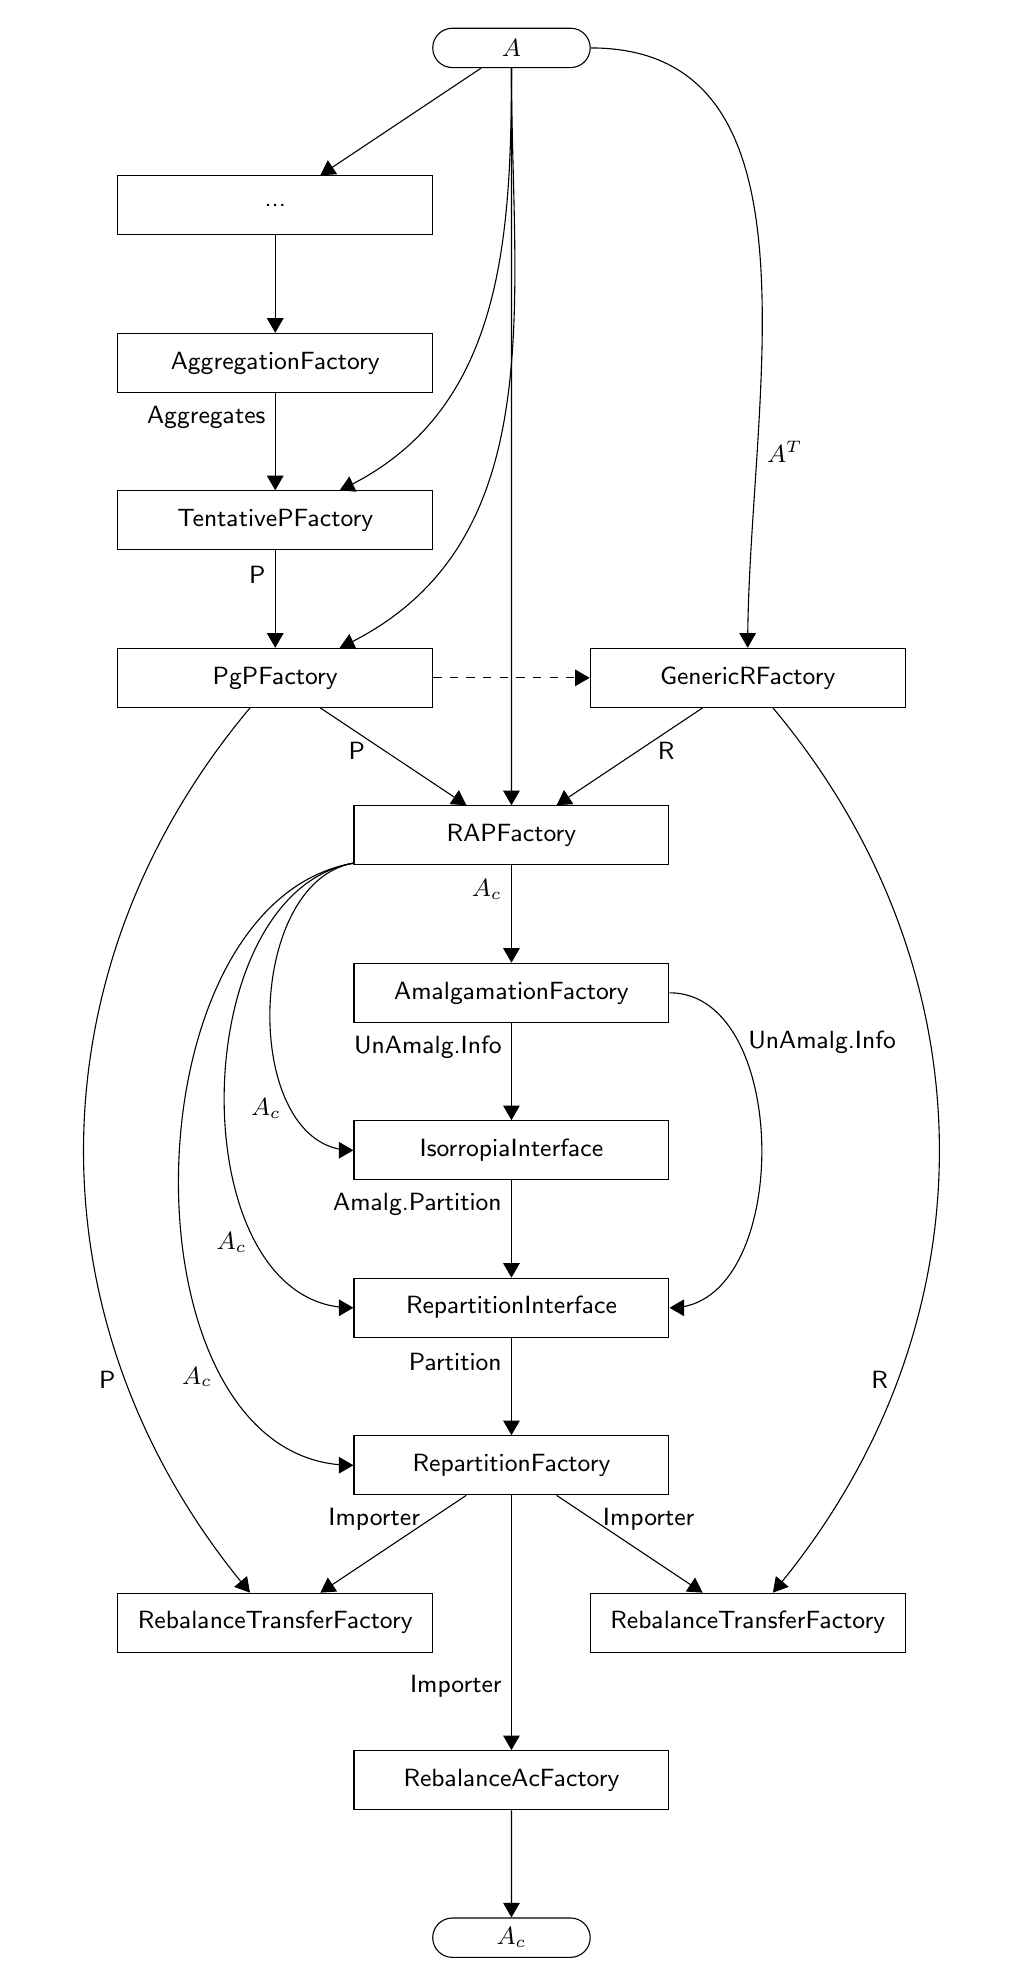
\begin{tikzpicture}[>=latex',font={\sf \small}, node distance=2cm]
\def\datawidth{2cm}
\def\dataheight{0.5cm}
\def\factorywidth{4cm}
\def\factoryheight{0.75cm}
%\draw[help lines] (-10,-10) grid (10,10);
\begin{scope}[>=triangle 60]
\node(A) at (0,10) [draw, terminal, minimum width=\datawidth, minimum height=\dataheight]{$A$};
\node(nothing) at (-3,8) [draw, process, minimum width=\factorywidth, minimum height=\factoryheight]{...};
\node [draw, process, minimum width=\factorywidth, minimum height=\factoryheight, below of=nothing] (AggregationFactory) {AggregationFactory};
\node [draw, process, minimum width=\factorywidth, minimum height=\factoryheight, below of=AggregationFactory] (TentativePFactory) {TentativePFactory};
\node [draw, process, minimum width=\factorywidth, minimum height=\factoryheight, below of=TentativePFactory] (SaPFactory) {PgPFactory};
\node [draw, process, minimum width=\factorywidth, minimum height=\factoryheight, right of=SaPFactory,node distance=6cm] (GenericRFactory) {GenericRFactory};
\node(RAPFactory) at(0,0) [draw, process, minimum width=\factorywidth, minimum height=\factoryheight]  {RAPFactory};

\node [draw, process, minimum width=\factorywidth, minimum height=\factoryheight, below of=RAPFactory] (RebAmalgFactory) {AmalgamationFactory};
\node [draw, process, minimum width=\factorywidth, minimum height=\factoryheight, below of=RebAmalgFactory] (IsorropiaInterface) {IsorropiaInterface};
\node [draw, process, minimum width=\factorywidth, minimum height=\factoryheight, below of=IsorropiaInterface] (RepartitionInterface) {RepartitionInterface};
\node [draw, process, minimum width=\factorywidth, minimum height=\factoryheight, below of=RepartitionInterface] (RepartitionFactory) {RepartitionFactory};
\node(RebalanceTransferFactory) at(-3,-10) [draw, process, minimum width=\factorywidth, minimum height=\factoryheight]  {RebalanceTransferFactory};
\node [draw, process, minimum width=\factorywidth, minimum height=\factoryheight, right of=RebalanceTransferFactory,node distance=6cm] (RebalanceTransferFactory2) {RebalanceTransferFactory};
\node(RebalanceAcFactory) at (0,-12) [draw, process, minimum width=\factorywidth, minimum height=\factoryheight]  {RebalanceAcFactory};

\node(A2) at (0,-14) [draw, terminal, minimum width=\datawidth, minimum height=\dataheight]{$A_c$};
\draw[->] (A) -- (nothing);
\draw[->] (nothing) -- (AggregationFactory);
\draw[->] (A) to[out=270,in=25] node [near start, left] {} (TentativePFactory);
\draw[->] (A) to[out=270,in=25] node [near start, left] {} (SaPFactory);
\draw[->] (A) to[out=270,in=90] node [near start, left] {} (RAPFactory);
\draw[->] (A) to[out=0,in=90] node [near end, right] {$A^T$} (GenericRFactory);
\draw[->] (AggregationFactory) -- node [near start, left] {Aggregates} (TentativePFactory);
\draw[->] (TentativePFactory) -- node [near start, left] {P} (SaPFactory);
\draw[->,dashed] (SaPFactory) -- node [near start, below] {} (GenericRFactory);
\draw[->] (SaPFactory) -- node [near start, below] {P} (RAPFactory);
\draw[->] (GenericRFactory) -- node [near start, below] {R} (RAPFactory);
%\draw[->] (RAPFactory) -- node [near start, below] {} (A2);
\draw[->] (RAPFactory) -- node [near start, left] {$A_c$} (RebAmalgFactory);
\draw[->] (RAPFactory) to[out=190,in=180] node [near end, left] {$A_c$} (IsorropiaInterface);
\draw[->] (RAPFactory) to[out=190,in=180] node [near end, left] {$A_c$} (RepartitionInterface);
\draw[->] (RAPFactory) to[out=190,in=180] node [near end, left] {$A_c$} (RepartitionFactory);
%\draw[->] (RAPFactory) to[out=190,in=180] node [near end, left] {$A_c$} (RebalanceAcFactory);
\draw[->] (RebAmalgFactory) -- node [near start, left] {UnAmalg.Info} (IsorropiaInterface);
\draw[->] (RebAmalgFactory) to[out=0,in=0] node [near start, right] {UnAmalg.Info} (RepartitionInterface);
\draw[->] (IsorropiaInterface) -- node [near start, left] {Amalg.Partition} (RepartitionInterface);
\draw[->] (RepartitionInterface) -- node [near start, left] {Partition} (RepartitionFactory);
\draw[->] (RepartitionFactory) -- node [near start, left] {Importer} (RebalanceTransferFactory);
\draw[->] (RepartitionFactory) -- node [near start, right] {Importer} (RebalanceTransferFactory2);
\draw[->] (RepartitionFactory) -- node [near end, left] {Importer} (RebalanceAcFactory);
\draw[->] (RebalanceAcFactory) -- node [near end, left] {} (A2);
\draw[->] (SaPFactory) to[out=230,in=130] node [near end, left] {P} (RebalanceTransferFactory);
\draw[->] (GenericRFactory) to[out=310,in=50] node [near end, left] {R} (RebalanceTransferFactory2);
\end{scope}
\end{tikzpicture}
} % end scalebox
\end{center}
\caption{Factory design for smoothed aggregation based algebraic multigrid methods for non-symmetric systems with rebalancing.}
\label{fig:rebalanceddesignpgamg}
\end{figure}

The XML parameters can be found in \verb|xml/s5a.xml|. Therein we define smoothed aggregation transfer operators (using the \verb|PgPFactory|) for non-sym\-metric systems. 1 sweep with an undamped symmetric Gauss-Seidel is used on the finest and intermedium levels. A direct solver is applied on the coarsest level. The intermedium multigrid levels are rebalanced.

\begin{graybox}
 \textbf{Exercise}
 \begin{itemize}
 \item Run the \verb|hands-on.sh| and choose either option 2 to set up a Laplace2D problem with a user-chosen mesh. Use reasonable values for \texttt{nx} and \texttt{ny}, e.g. \verb|nx=300| and \verb|ny=300|.
 \item Change the solver (using option 4) to \verb|xml/s5a.xml|.
 \item Use a reasonable number of processors (option 5). For demonstration purposes $4$ processors should be fine for the $300\times 300$ mesh.
 \item Adapt the \verb|numprocs| variable in the \verb|MueLu_Agg2VTK.py| postprocessing script. Rerun the example (option 1) and make sure that \verb|MueLu_Agg2VTK.py| is executed afterwards (should be done automatically).
 \item Use \verb|paraview| to visualize the aggregates. Open \verb|paraview| and load the \verb|aggs*.vtp| files. Use the processor id as colors.
 \item Repeat above steps for the Recirc2D example. Vary the \verb|minRowsPerProcessor| and \verb|nonzeroImbalance| parameters.
 \end{itemize}
\end{graybox}

\begin{figure}
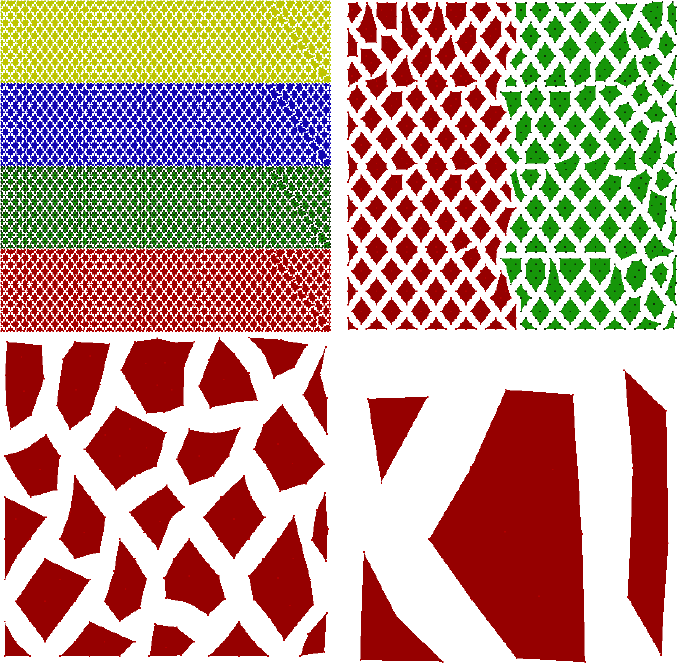
\includegraphics[width=\textwidth]{images/aggsSymmReb.png} 
\caption{Aggregates and owning processors for level 1 to level 4 for a 2D Laplace problem on a $300\times 300$ mesh}
\label{fig:rebAggs}
\end{figure}

Figure \ref{fig:rebAggs} shows the aggregates and the owning processors for the different multigrid levels. One can see how the number of involved processors is reduced and how it affects the shape of aggregates.


\section{Tutorial 6}

In this tutorial we want to introduce the C++ API of \MueLu. We write a small test program for the \verb|Recirc2D| example as introduced in the first example, but instead of building the multigrid hierarchy using an xml parameter file we use the C++ routines to define the multigrid method.

\subsection{Test program}
The source code of the test program can be found in \verb|recirc2d_api.cpp|. Most of the source code is not relevant for this tutorial. First, the parallel environment is initialized and some parameters are read from the command line. Then the linear system is generated using the \verb|Galeri| package from Trilinos. The linear system has to be transformed to \Xpetra~ objects, that are needed by \MueLu. Supposing that we have the fine level matrix $A$ and a null space vector we can build the multigrid method.
Note, that we are using the refrence-counted pointers from the \verb|Teuchos| package in Trilinos. The so-called \verb|RCP| pointers automatically free used memory as soon as the underlaying object is destroyed. This simplifies programming a lot and avoids memory leaks\footnote{See http://trilinos.sandia.gov/RefCountPtrBeginnersGuideSAND.pdf for an introduction to RCP pointers.}

\paragraph{Create Multigrid hierarchy.}
The central part of the multigrid setup phase is given in listing \ref{listing:CppAPI}.
In line 1 we create a new Hierarchy object, which stores the multigrid hiearchy and provides the basic functionality for a multigrid method, such as a V cycle or a W cycle. Next we set some basic parameters of the multigrid hierarchy, such as the maximum coarse level size and the verbosity level for debug output.

\paragraph{Define finest level object.}
The second step is to define and fill the finest level object with the initial information. The Hierarchy object, that has been generated above provides an empty level that is returned by the \verb|GetLevel| function. Then we store the finest level matrix $A$ as variable "A" and the fine level null space vector as variable "Nullspace" in the Level object using the \verb|Set| member function.

\paragraph{Define a factory collection.}
The next step is to define the factory collection and create instances of all factories that we wanna use to replace the internal default factories. For demonstration purposes we want to create a multigrid hierarchy with non-smoothed transfer operators. % and a symmetric Gauss-Seidel method as multigrid smoother on all multigrid levels.
Since the \MueLu default settings define a smoothed aggregation prolongation operator with the transposed of the smoothed prolongator as restriction operator, we just have to "overwrite" the prolongation factory as it is done in line 14 of listing \ref{listing:CppAPI}. There we create our own instance of a tentative non-smoothed prolongation factory and store it in the local variable \verb|PFact|. Later we will show how to register our \verb|PFact| instance of the non-smoothed prolongation operator in the multigrid hierarchy setup routine.

For demonstration purposes we create an instance of the \verb|TransPFactory| to generate the restriction operator, too. With the line
\begin{verbatim}
RFact->SetFactory("P", PFact);
\end{verbatim}
we declare the variable "P" generated by our non-smoothed prolongation operator factoy \verb|PFact| as input prolongator that is to be used to calculate the restriction operator by building the transpose. In general you use the \verb|SetFactory| member function to declare the input variables of a factory. The first parameter gives the name of the input variable and the second prameter the generating factory object of the variable. The \verb|SetFactory| member function is very useful to explicitely declare the input variables and factories for a given factory. If you don't declare the input variables \MueLu~ will try to use default factories to generate the necessary input data or - in the worst case - will fail if it is not able to generate the needed data using the default factories.

It should be rather simple to build the factory collection if you have the corresponding XML parameter file or a picture of the factory design (as e.g. in figure \ref{fig:simpledesignnonsmoothed}). The building blocks correspond to the factory instances and the arrows in between the building blocks are defined by corresponding \verb|SetFactory| calls. If you have the XML parameter files, then the parameters with the name "factory" give the class name of the factory class (e.g. \verb|SaPFactory|). All other parameters with different names usually define the arrows between the factories.

\paragraph{Setup level smoothers.}
For the level smoothers \MueLu~ uses the prototype design pattern \footnote{see e.g. http://en.wikipedia.org/wiki/Prototype\_pattern}. 
We create a new \verb|TrilinosSmoother| prototype object which is fed by a parameter list with all necessary parameters (e.g. for a Symmetric Gauss-Seidel smoother). A list of all possible parameters can be found in the class documentation.
The prototype object then is used as parameter for the \verb|SmootherFactory| instance. In each multigrid level the smoother factory then creates a new instance of the level smoother based on the information from the prototype class.

\paragraph{The FactoryManager}
The \verb|FactoryManager| object is the heart of the multigrid setup phase since it manages all the dependencies between the factories. The default implementation automatically creates factories which are necessary to build a multigrid hierarchy for symmetric positive definite systems (with smoothed aggregation transfer operators etc...). The user can change this default behaviour by defining new factories (see above) and registering them in the \verb|FactoryManager| object. In listing \ref{listing:CppAPI} line 34-39 a \verb|FactoryManager| object is created and the previously defined factories for the transfer operators and smoothers are registered as default factories for the variables "P", "R", "Nullspace", "Smoother" and "CoarseSolver" using the \verb|SetFactory| function.

If we register the new factories as default factories in the \verb|FactoryManager| object most of the factory specific connections are not necessary any more. For example in listing \ref{listing:CppAPI} we could remove line 16, since then the \verb|TransPFactory| woudl use the object with name "P" that is generated by the default factory which is again \verb|PFact| as defined in line 14 and registered as default factory in line 37. We could also remove line 36, since the \verb|FactoryManager| in its default implementation would automatically generate an \verb|TransPFactory| instance for building the restriction operator. In this case, our \verb|TransPFactory| instance defined in line 15 would be created but never used. It is not registered in the factory manager and therefore not involved in the setup process.

In general it is a good idea to rely on the factory manager rather on defining all factories by hand. Often one forgets some factories or connections between factories resulting in hard-to-debug inconsistencies between the default factories in the factory manager and some lost factories in the factory collection. The factory manager makes it easy to generate a consistent set of factories for the multigrid setup phase.

\paragraph{Build the multigrid hierarchy}
Last but not least, the multigrid hiearchy is built by the simple call
\begin{verbatim}
H->Setup(M, 0, maxLevels);
\end{verbatim}
where \verb|M| is the factory manager and the other parameters define the level id of the finest level and the maximum number of allowed multigrid levels.
The generated hierarchy then can be used as solver or preconditioner within a Krylov method. Corresponding code snippets how to do this can be found in the example program in \verb|recirc2d_api.cpp|.

\begin{Listing}
\begin{center}
\begin{lstlisting}[language=c++]
  RCP<Hierarchy> H = rcp ( new Hierarchy() );
  H->setDefaultVerbLevel(Teuchos::VERB_HIGH);
  H->SetMaxCoarseSize(maxCoarseSize);
  H->setlib(Xpetra::UseEpetra);

  // build finest Level
  RCP<MueLu::Level> Finest = H->GetLevel();
  Finest->setDefaultVerbLevel(Teuchos::VERB_HIGH);
  Finest->setlib(Xpetra::UseEpetra);
  Finest->Set("A",A);
  Finest->Set("Nullspace",nullspace);

  // create factories for transfer operators
  RCP<TentativePFactory> PFact = Teuchos::rcp(new TentativePFactory());
  RCP<TransPFactory>     RFact = Teuchos::rcp(new TransPFactory());
  RFact->SetFactory("P", PFact);

  // build level smoothers
  // use symmetric Gauss-Seidel both for fine and coarse level smoother
  RCP<SmootherPrototype> smooProto;
  std::string ifpackType;
  Teuchos::ParameterList ifpackList;
  ifpackList.set("relaxation: sweeps", (LO) 1);
  ifpackList.set("relaxation: damping factor", (SC) 1.0);
  ifpackType = "RELAXATION";
  ifpackList.set("relaxation: type", "Symmetric Gauss-Seidel");

  smooProto = Teuchos::rcp( new TrilinosSmoother(ifpackType, ifpackList) );
  RCP<SmootherFactory> SmooFact;
  if (maxLevels > 1)
    SmooFact = rcp( new SmootherFactory(smooProto) );

  // design multigrid hierarchy
  FactoryManager M;
  M.SetFactory("P", PFact);
  M.SetFactory("R", RFact);
  M.SetFactory("Nullspace", PFact);
  M.SetFactory("Smoother", SmooFact);
  M.SetFactory("CoarseSolver", SmooFact);

  H->Setup(M, 0, maxLevels);
\end{lstlisting}
\caption{C++ API for defining multigrid hierarchy.} 
\label{listing:CppAPI}
\end{center}
\end{Listing}

\begin{graybox}
 \textbf{Exercise}
 \begin{itemize}
  \item The \verb|FactoryManager| per default uses a \verb|CoupledAggregationFactory| strategy. Often there are many good reasons to switch to the \verb|UncoupledAggregationFactory|. Extend the test program in \verb|Recirc2d_api.cpp| to use uncoupled aggregation instead of coupled aggregation. Use the \verb|SetParameter| member function to set internal variables in the \verb|UncoupledAggregationFactory| class, such as \verb|MinNodesPerAggregate|:
  \begin{verbatim}
  RCP<UncoupledAggregationFactory> UCAggFact = 
                rcp(new UncoupledAggregationFactory());
  UCAggFact->SetParameter("MinNodesPerAggregate",
                   Teuchos::ParameterEntry(minPerAgg));
  \end{verbatim}
  The general rule for all factory classes is: the list of all valid parameters is located in the \verb|GetValidParameterList()| member function\footnote{Find the parameters of the uncoupled aggregation strategy e.g. in packages/muelu/src/Graph/UncoupledAggregation/MueLu\_UncoupledAggregationFactory\_def.hpp.}.
  \item Of course, we do not want to set the prolongation operator smoothing aside. Since it is a non-symmetric problem we choose the Petrov-Galerkin approach together with the flexible prolongation operator smoothing strategy from the \verb|PgPFactory|. Extend the test program by a \verb|PgPFactory| instance for prolongation smoothing. Use the tentative prolongation factory \verb|PFact| as input for the \verb|PgPFactory|. For the Petrov-Galerkin transfer operator smoothing approach switch from \verb|TransPFactory| to the \verb|GenericRFactory|. Set the factory dependencies accoordingly and update the factory manager.
  \item Introduce an option to use the smoothed prolongation operator (generated by the \verb|PgPFactory|) together with a non-smoothed restriction operator (the transpose of the output of the \verb|TentativePFactory|). Note, that the \verb|GenericRFactory| does not accept a \verb|TentativePFactory| as input. For that case, use a \verb|TransPFactory| instead.
 \end{itemize}
\end{graybox}


\begin{thebibliography}{9}
\bibitem{vanek1996} Vanek, P. and Mandel, J. and Brezina, M. Algebraic Multigrid by Smoothed Aggregation for Second and Fourth Order Elliptic Problems, Computing, 1996, 56, p. 179--196
\bibitem{sala2008} Sala, M. and Tuminaro, R. S., A new Petrov-Galerkin Smoothed Aggregation Preconditioner for nonsymmetric Linear Systems, SIAM J. Sci. Comput., 2008, 31, p. 143--166
\bibitem{wiesner2013} Wiesner, T. A., Tuminaro, R. S., Wall, W. A. and Gee, M. W., Multigrid transfers for nonsymmetric systems based on Schur complements and Galerkin projections., Numer. Linear Algebra Appl., 2013, doi: 10.1002/nla.1889
%\bibitem{hackbusch1994} Wolfgang Hackbusch, Iterative Solution of Large Sparse Systems of Equations, Springer, New York, 1994.
%\bibitem{saad2005} Yousef Saad, Multilevel ILU with reorderings for diagonal dominance, SIAM J. Sci. Comput, 2005, vol. 27.
%\bibitem{duff1999} I.S. Duff and J. Koster, The design and use of algorithms for permuting large entries to the diagonal of sparse matrices, SIAM J. Matrix Anal. Appl., 1999, vol. 20, p. 889--901.
\end{thebibliography}

\end{document}